\documentclass[10pt, letterpaper]{report}
% !TeX program = xelatex
%==================PREAMBOLO=======================%
\usepackage[utf8]{inputenc}
\usepackage{psvectorian}
\usepackage{pgfplots}
\usepackage[Rejne]{fncychap}
\usepackage[export]{adjustbox}
\usepackage[T1]{fontenc}
\usepackage{lmodern}
\usepackage{blindtext}
\usepackage{pdfpages}
\usepackage[shortlabels]{enumitem}
\usepackage{moresize}
\usepackage{graphicx} % Required for inserting images
\usepackage{hyperref}
\usepackage{listings}
\usepackage[table,xcdraw]{xcolor}
\usepackage{amssymb}
\usepackage{amsmath}
\usepackage[english]{babel}
\usepackage{nicefrac, xfrac}
\usepackage{tikz}
\usepackage{tikz-3dplot}
\usepackage{tikz-cd}
\usepackage{mathrsfs} 
\usepackage{titletoc}
\usepackage{fancyhdr}
\usepackage{psvectorian,lipsum}
\usepackage{fourier-orns}
\usepackage{lipsum}
\usepackage{wrapfig}
\usepackage{multicol}
\usepackage[paper=a4paper,left=25mm,right=25mm,bottom=25mm,top=25mm]{geometry}
\definecolor{light-gray}{gray}{0.95}
\definecolor{cop}{HTML}{f7ecd7}
\definecolor{copAut}{HTML}{ababab}
\definecolor{copAut2}{HTML}{c3c3e6}
\definecolor{purcop}{HTML}{d0d3db}
\definecolor{sapienza}{HTML}{660f1d}
\definecolor{lightSapienza}{HTML}{e3d3d5}
\definecolor{darkgreen}{HTML}{008000}
\definecolor{cartaRiciclata}{HTML}{fcfcf7}
\newcommand{\redText}[1]{\color{red}#1\color{black}}
\newcommand{\code}[1]{\colorbox{light-gray}{\texttt{#1}}}
\newcommand{\codee}[1]{\colorbox{white}{\texttt{#1}}}
\newcommand{\K}{{\mathbb K}}
\newcommand{\notimplies}{%
  \mathrel{{\ooalign{\hidewidth$\not\phantom{=}$\hidewidth\cr$\implies$}}}}
\newcommand{\flowerLine}{ \begin{center}\decofourleft\hphantom{ }\decoone\hphantom{ }\decofourright\hphantom{}\hphantom{aa}
\decofourleft\hphantom{ }\decoone\hphantom{ }\decofourright\hphantom{}\hphantom{aa}
\decofourleft\hphantom{ }\decoone\hphantom{ }\decofourright\hphantom{}\hphantom{aa}
\decofourleft\hphantom{ }\decoone\hphantom{ }\decofourright\hphantom{}\hphantom{aa} 
\decofourleft\hphantom{ }\decoone\hphantom{ }\decofourright\hphantom{}\hphantom{aa}
\decofourleft\hphantom{ }\decoone\hphantom{ }\decofourright\hphantom{}\hphantom{aa}
\decofourleft\hphantom{ }\decoone\hphantom{ }\decofourright\hphantom{}\hphantom{aa}
\decofourleft\hphantom{ }\decoone\hphantom{ }\decofourright\hphantom{}\hphantom{aa}
\decofourleft\hphantom{ }\decoone\hphantom{ }\decofourright\hphantom{}\hphantom{aa}
\end{center}}
\definecolor{g}{RGB}{60, 50, 50}
\newcommand{\textg}[1]{\color{g}{\textbf{#1}}\color{black}}
\newcommand{\teo}[1]{{\large\color{sapienza}\textbf{Teorema #1 :\hphantom{a}}}}
\newcommand{\defi}[1]{{\large\color{sapienza}\textbf{Definizione #1 :\hphantom{a}}}}
\newcommand{\claim}[1]{{\color{sapienza}\textbf{Claim #1 :\hphantom{a}}}}
\newcommand{\lemma}[1]{{\color{sapienza}\textbf{Lemma #1 :\hphantom{a}}}}
\newcommand{\dimo}[1]{{\color{sapienza}\textbf{Dimostrazione #1 :\hphantom{a}}}}
\newcommand{\prop}[1]{{\color{sapienza}\textbf{Proposizione #1 :\hphantom{a}}}}
\newcommand\greybox[1]{%
  \vskip\baselineskip%
  \par\noindent\colorbox{light-gray}{%
    \begin{minipage}{\textwidth}#1\end{minipage}%
  }%
  \vskip\baselineskip%
}
\newcommand\sapbox[1]{%
  \vskip\baselineskip%
  \par\noindent\colorbox{lightSapienza}{%
    \begin{minipage}{\textwidth}#1\end{minipage}%
  }%
  \vskip\baselineskip%
}
\newcommand{\ridFunc}{{f:\Sigma^*\rightarrow \Sigma^*}}
\newcommand{\rid}{{\le_m^P}}
\newcommand{\Z}{{\mathbb Z}}
\newcommand{\blank}{{\sqcup}}
\newcommand{\Prob}{{\mathbb P}}
\newcommand{\R}{{\mathbb R}}
\newcommand{\VA}{{\mathbb E}}
\newcommand{\btheta}{{\boldsymbol{\theta}}}
\newcommand{\bomega}{{\boldsymbol{\omega}}}
\newcommand{\N}{{\mathbb N}}
\newcommand{\quat}{{\mathbb H}}
\newcommand{\C}{{\mathbb C}}
\newcommand{\Sn}{{\mathcal S_n}}
\newcommand{\An}{{\mathcal A_n}}
\newcommand{\E}{{\mathcal E}}
\newcommand{\B}{{\mathcal B}}
\newcommand{\mcm}{{\text{mcm}}}
\newcommand{\rg}{{\text{rg}}}
\newcommand{\ve}{{\bar v}}
\newcommand{\spaz}{{\text{\hphantom{aa}}}}
\newcommand{\MCD}{{\text{MCD}}}
\newcommand{\tc}{{\text{ tale che }}}
\newcommand{\supp}{{\text{Supp}}}
\newcommand{\acc}{\\\hphantom{}\\}
\newcommand{\esempio}[1]{{\acc\large\color{sapienza}\textbf{Esempio #1 \hphantom{a}}\acc}}
\newcommand{\bra}[1]{\langle #1 \rangle}
\newcommand{\aut}{{\text{Aut}}}
\newcommand{\Span}{{\text{Span}}}
\newcommand{\End}{{\text{End}}}
\newcommand{\cen}{{\text{Centro}}}
\newcommand{\norm}{{\unlhd}}
\newcommand{\ciclS}{{\left \langle }}
\newcommand{\ciclE}{{\right \rangle }}
\newcommand{\boxedMath}[1]{\begin{tabular}{|c|}\hline \texttt{#1} \\ \hline\end{tabular} :} 
\newcommand{\shell}[1]{\colorbox{black}{\textcolor{white}{\texttt{#1}}}}
\newcommand{\eqImportante}[1]{\begin{center}\huge\lefthand\hphantom{a}
    \normalsize\texttt{#1}
    \hphantom{aaa}\huge\righthand\end{center}}

\fancyhf{}
\pagestyle{fancy}
\usepackage{pgf-pie}  
\usetikzlibrary{positioning}

\renewcommand{\headrule}{%
\vspace{-8pt}\hrulefill
\raisebox{-2.1pt}{\quad\decothreeleft\decotwo\decothreeright\quad}\hrulefill}

%sta roba serve per il codice C
\definecolor{mGreen}{rgb}{0,0.6,0}
\definecolor{mGray}{rgb}{0.5,0.5,0.5}
\definecolor{mPurple}{rgb}{0.58,0,0.82}
\definecolor{backgroundColour}{rgb}{0.95,0.95,0.92}

\lstdefinestyle{CStyle}{
    backgroundcolor=\color{backgroundColour},   
    commentstyle=\color{mGreen},
    keywordstyle=\color{magenta},
    numberstyle=\tiny\color{mGray},
    stringstyle=\color{mPurple},
    basicstyle=\footnotesize,
    breakatwhitespace=false,         
    breaklines=true,                 
    captionpos=b,                    
    keepspaces=true,                 
    numbers=left,                    
    numbersep=5pt,                  
    showspaces=false,                
    showstringspaces=false,
    showtabs=false,                  
    tabsize=2,
    language=C
}
\lstdefinestyle{CppStyle}{
    backgroundcolor=\color{backgroundColour},   
    commentstyle=\color{mGreen}\ttfamily,
    morecomment=[l][\color{magenta}]{\#}
    keywordstyle=\color{blue}\ttfamily,
    numberstyle=\tiny\color{mGray},
    stringstyle=\color{red}\ttfamily,
    basicstyle=\ttfamily,
    breakatwhitespace=false,         
    breaklines=true,                 
    captionpos=b,                    
    keepspaces=true,                 
    numbers=left,                    
    numbersep=5pt,                  
    showspaces=false,                
    showstringspaces=false,
    showtabs=false,                  
    tabsize=2,
    language=C
}
\lstset{language=C++,
                basicstyle=\ttfamily,
                keywordstyle=\color{blue}\ttfamily,
                stringstyle=\color{red}\ttfamily,
                commentstyle=\color{green}\ttfamily,
                morecomment=[l][\color{magenta}]{\#}
}
%fine roba che serve per il codice C
\usepackage{minted}
\usepackage{algorithm}
\usepackage{algpseudocode}
\usepackage{booktabs}
\newcommand{\titolo}{Machine Learning }

 %TOGLI COMMENTO SE USI XELATEX
%\usepackage{fontspec}
\title{\titolo} %========TITOLO========%
\author{Marco Casu, Claudio Loriga}
\date{\vspace{-5ex}}
\begin{document}

%==================COPERTINA=======================%
\begin{titlepage}

	\vfill
	\centering 
\includegraphics[width=0.4\textwidth ]{preamble/Stemma_sapienza.png} \acc
	\centering \Large {\color{sapienza}Faculty of Information Engineering, Computer Science and Statistics\\
		Department of Computer, Control and Management Engineering\\
		Master's degree in Artificial Intelligence and Robotics}
	\bigskip
	\begin{center}
		%TOGLI COMMENTO SE USI XELATEX
		%\setmainfont{Palace Script MT}
		\HUGE Marco Casu, Claudio Loriga\acc
	\end{center}
	\thispagestyle{empty}
	\begin{figure}[h]
		\centering{
			%l'immagine deve avere una risoluzione 2048x2048
			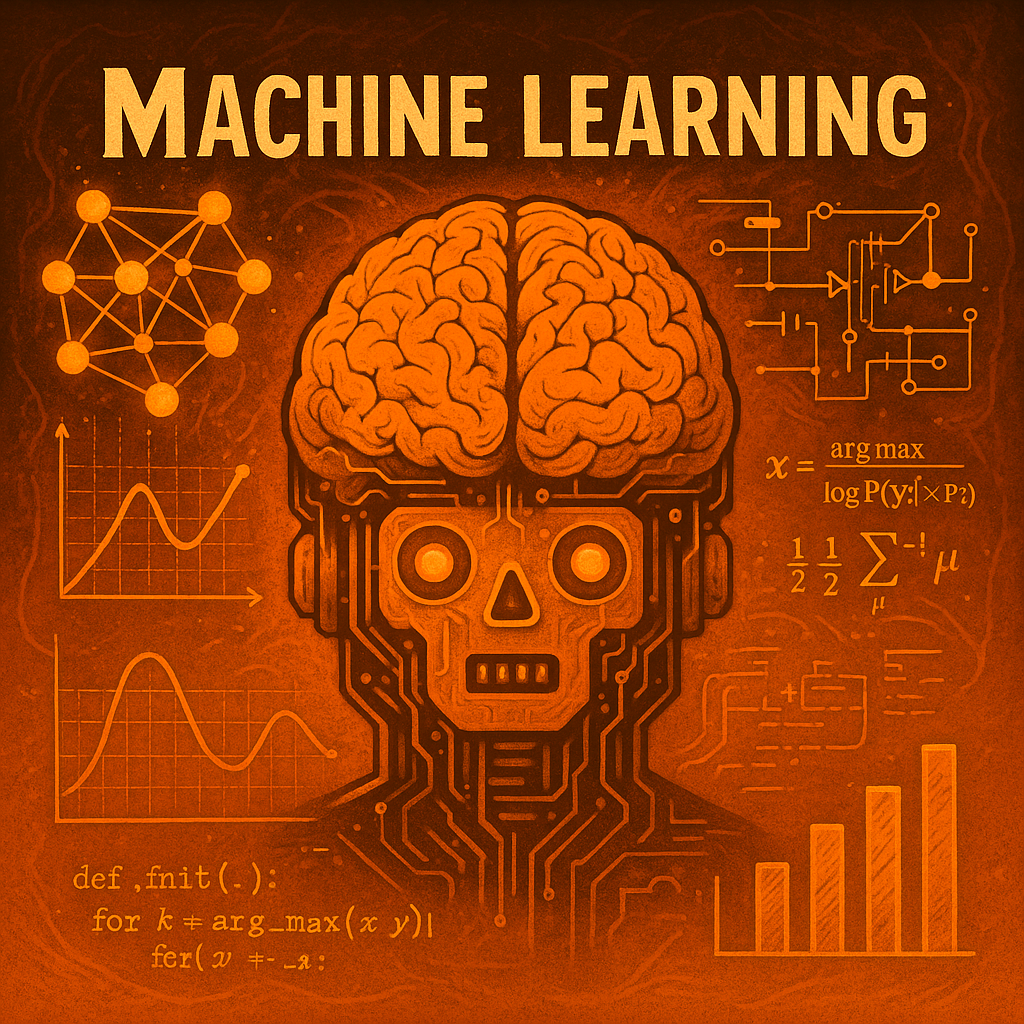
\includegraphics[width=1\textwidth ]{images/CopertinaNew.png}
		}
	\end{figure}
\end{titlepage}

%===================FINE COPERTINA======================%
\newpage
%\pagecolor{cartaRiciclata}%\setmainfont{Algerian}
\Large
This document summarizes and presents the topics for the
\titolo course for the Master's degree in Artificial Intelligence
and Robotics at Sapienza University of Rome. The document is free for any use.
If the reader notices any typos, they are kindly requested to report them to the author.
Additionally, Claudio decided to edit this document has been edited to try give an emphasis
on arguments which are sensible to subjects with basic mathematical skills (like me :D)
\vfill
\begin{figure}[h!]
	\raggedright
	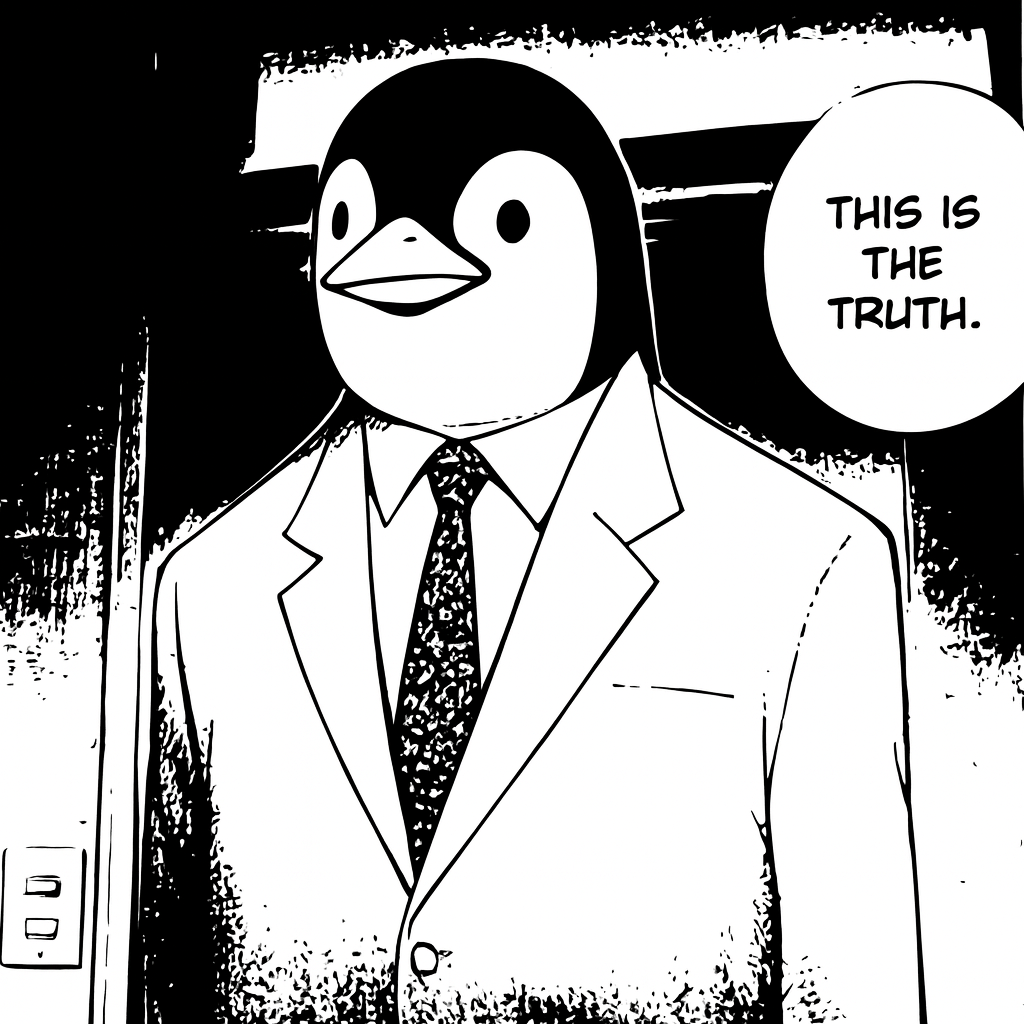
\includegraphics[width=0.4\textwidth,right ]{images/PenguinTruth.png}
\end{figure}
\newpage %\setmainfont{Times New Roman}
\normalsize

\tableofcontents
\newpage

%==================FOOTER e HEADER=======================%
\fancyhf{}
\fancyhead[L]{\nouppercase{\leftmark}}
\fancyhead[R]{Sezione \thesection}
\fancyfoot[C]{\thepage}
\fancyfoot[L]{\titolo}
\fancyfoot[R]{ Marco Casu, Claudio Loriga}
%\fancyfoot[R]{\setmainfont{Palace Script MT}\huge Marco Casu \setmainfont{Times New Roman}}
%==================FOOTER e HEADER=======================%

\newtheorem{definition}{Definition}
\newtheorem{theorem}{Theorem}
%==================INIZIO======================%
\chapter{Introduction}

\section{Basic Definition of a ML Problem}
In this chapter, we will introduce the fundamental ideas behind machine learning (ML) — what it is, why it matters, and how we can formally describe a learning problem.\bigskip

At its core, machine learning is the \textbf{study of computer systems that improve their performance on a given task through experience}.
Rather than being explicitly programmed with a fixed set of rules, an ML system \textbf{learns patterns and behaviors from data, adapting its internal model to make predictions, recognize structures, or take actions in complex environments.}\bigskip

Machine learning lies at the intersection of computer science, statistics, and optimization, providing methods that allow computers to make sense of data — whether that means classifying images, predicting financial trends, generating text, or controlling autonomous vehicles.\bigskip

From a more formal perspective, a learning problem can be described by three components:\begin{itemize}
	\item $T$ : the \textbf{task} we want the system to perform,
	\item $P$ : a \textbf{performance measure} that quantifies how well the system performs the task, and
	\item $E$ : the experience or \textbf{data} from which the system learns.
\end{itemize}

The goal of learning is to improve performance P on task T by using experience E.\bigskip

Let's see an example, we want to model a program capable of playing \textit{Checkers}.
\begin{center}
	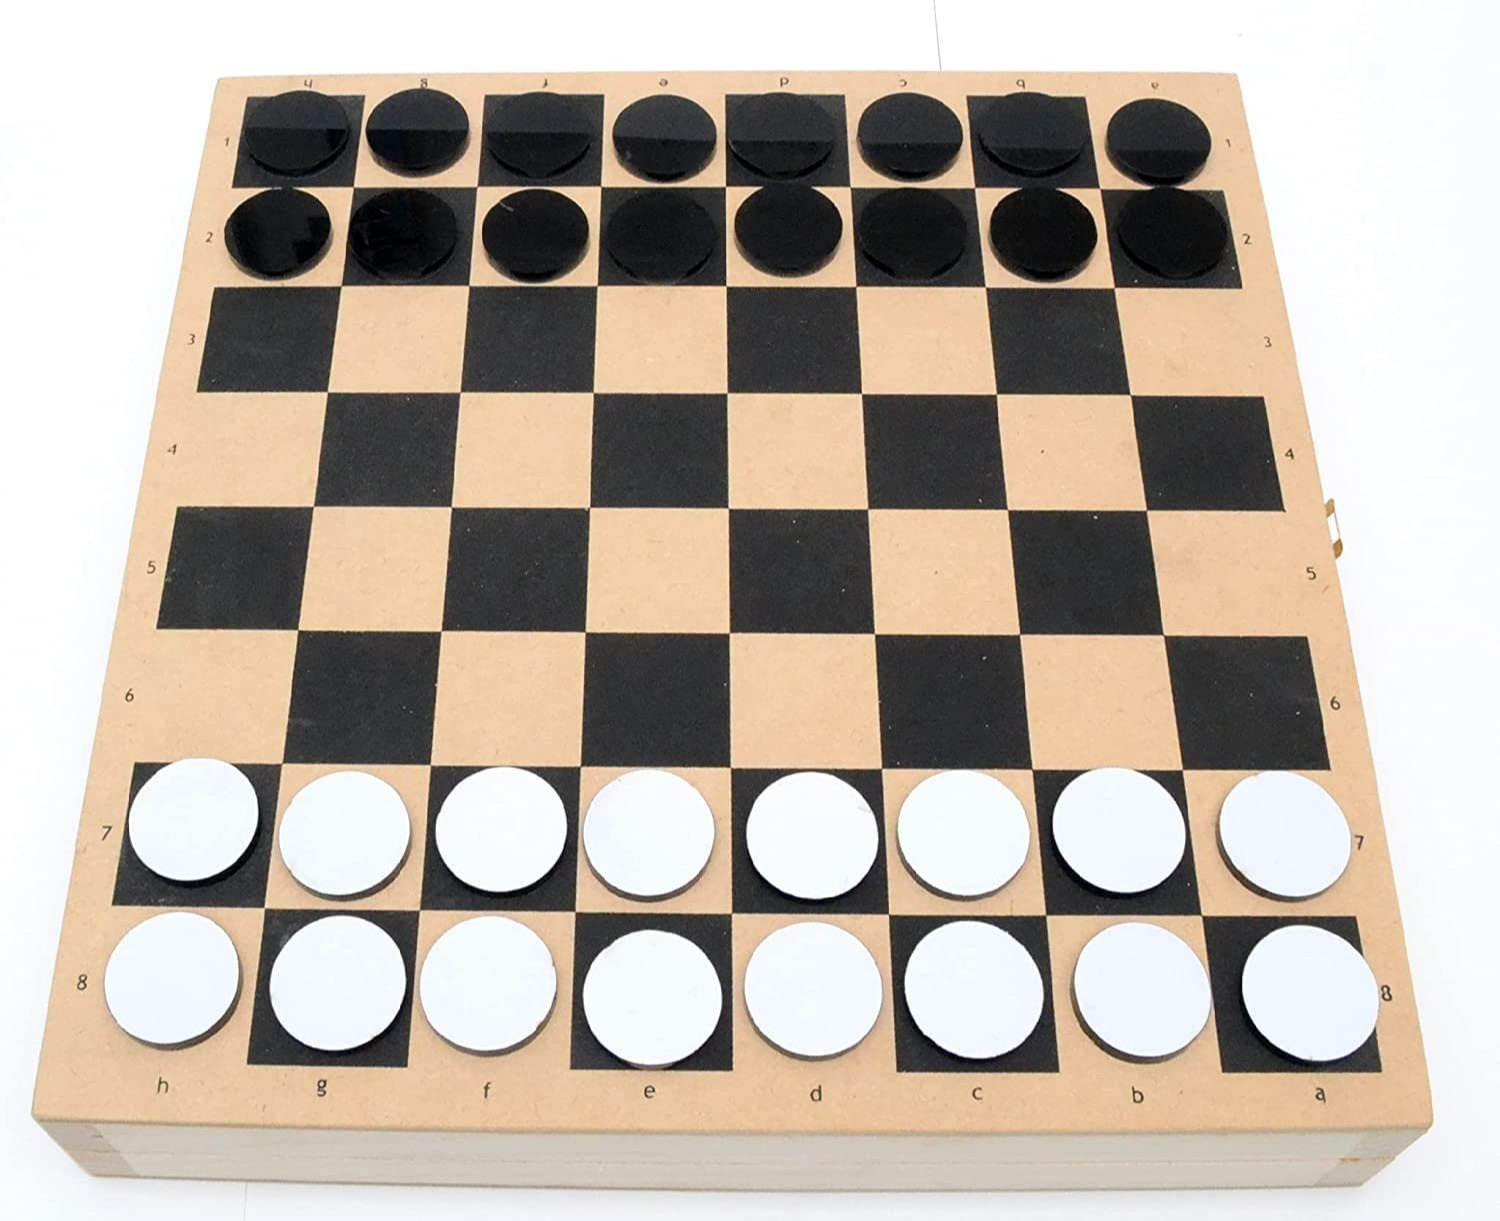
\includegraphics[width=0.35\textwidth]{images/Checkers.jpg}
\end{center}
The task $T$ is to play the game of Checkers. The performance metric $P$ measures the ratio of wins in a tournament, and the experience $E$ is given by the outcomes of past matches. These matches can be generated either by letting the program play against itself (self–play) or by recording games against human opponents. We can formalize the agent’s behaviour through two types of target functions:
\begin{itemize}
	\item $ChooseMove : Board \rightarrow Move$
	\item $V : Board \rightarrow \R$
\end{itemize}
Here, $Board$ is the set of all possible board configurations and $Move$ is the set of feasible moves. The image of the value function $V$ should represent how favorable a position is for the player:
\begin{itemize}
	\item if $b\in Board$ is a configuration that represents a win for the player, then $V(b)=1$;
	\item if $b\in Board$ is a configuration that represents a win for the opponent, then $V(b)=-1$;
	\item if $b\in Board$ is a configuration that represents a draw, then $V(b)=0$;
	\item otherwise, $V(b)=V(b')$ where $b'$ is the best final board state that can be achieved starting from $b$ assuming both players play optimally until the end of the game.
\end{itemize}

The function $V$ can be used to select the next move by evaluating all boards reachable from the current position and choosing the move that maximizes $V$. However, $V$ is an \emph{idealized} object: it assumes we already know what ``optimal play'' is, so it is not computable in practice. Our goal, therefore, is to \emph{approximate} $V$ with a function we can learn from data.

\bigskip
\textbf{Approximating the value function:}
We consider a parametric approximation $\hat V: Board\rightarrow\R$ of the form
\begin{equation}
	\hat V(b)=\sum_{i=0}^6 w_i\, f_i(b),
\end{equation}
where $\mathbf w=(w_i)$ are real coefficients to be learned, and the $f_i$ are \emph{features} of the board $b$, for example:
\begin{itemize}
	\item $f_1(b)$: number of black pieces on $b$,
	\item $f_2(b)$: number of red pieces on $b$,
	\item etc.
\end{itemize}
Not all features are equally informative. The quality of $\hat V$ depends heavily on choosing features that capture meaningful aspects of the position (domain knowledge).

\bigskip
\textbf{Learning from data:}
By \emph{learning the function} $\hat V$ we mean finding coefficients $\mathbf w$ that make $\hat V$ as close as possible to $V$ on the available data. Let us introduce some notation:
\begin{itemize}
	\item $V$: the (unknown and uncomputable) \textbf{target function};
	\item $\hat V$: the \textbf{learned function}, our approximation to $V$;
	\item $V_{\text{train}}(b)$: the target value provided by the dataset for board $b$;
	\item $D$ (dataset):
	      \begin{equation}
		      D=\bigcup_{i=1}^n\{(b_i,\, V_{\text{train}}(b_i))\},
	      \end{equation}
	      where $n$ is the number of available samples.
\end{itemize}

The following iterative rule (Algorithm~\ref{alg:LMS}) informally illustrates how we can update $\mathbf w$.

\begin{algorithm}
	\caption{LMS weight update rule}\label{alg:LMS}
	\begin{algorithmic}
		\Require $D$, $V_{\text{train}}$, $k$
		\State initialize $\mathbf w$ with small random values
		\For{$k$ times}
		\State select a sample $b$ from $D$
		\State $error(b)=V_{\text{train}}(b)-\hat V(b)$
		\For{each feature $i$}
		\State $w_i\leftarrow w_i + c \cdot f_i(b) \cdot error(b)$
		\EndFor
		\EndFor
	\end{algorithmic}
\end{algorithm}

Here $c\in(0,1]$ is the \emph{learning rate}, which moderates how quickly the model adapts.

\bigskip
\textbf{What the error signal means (and why it works):}
The term
\[
	error(b)=V_{\text{train}}(b)-\hat V(b)
\]
quantifies the discrepancy between the desired value and the model’s current prediction for board $b$. It acts as a feedback signal:
\begin{itemize}
	\item if $\hat V(b)$ is \emph{too small}, $error(b)>0$ and the update increases those weights $w_i$ whose features $f_i(b)$ are active, pulling $\hat V(b)$ upward on similar positions;
	\item if $\hat V(b)$ is \emph{too large}, $error(b)<0$ and the update decreases the corresponding weights, pushing $\hat V(b)$ downward.
\end{itemize}
Repeated over many samples, these nudges steer $\mathbf w$ toward values that reduce the overall discrepancy on the dataset.

Formally, LMS can be seen as (a stochastic) gradient step that aims to minimize the \emph{sum of squared errors}:
\begin{equation}
	\label{eq:sse_objective}
	\sum_{b_i\in D} \bigl( V_{\text{train}}(b_i)-\hat V(b_i)\bigr)^2.
\end{equation}
(Using the square makes large mistakes count more and yields a smooth objective; the update above corresponds to a gradient step on \eqref{eq:sse_objective} for a linear $\hat V$.)

\bigskip
\textbf{Closing the loop with new experience.}
Once we have synthesized $\hat V$, we can let the model play new games (against humans or via self–play), record the outcomes, and add these to $D$. This enlarges the experience $E$ and enables another round of learning, creating an \emph{iterative improvement loop}. The diagram in Figure~\ref{img:DesignChoice} summarizes this design process for an intelligent agent.

\bigskip
\begin{figure}[h!]
	\centering
	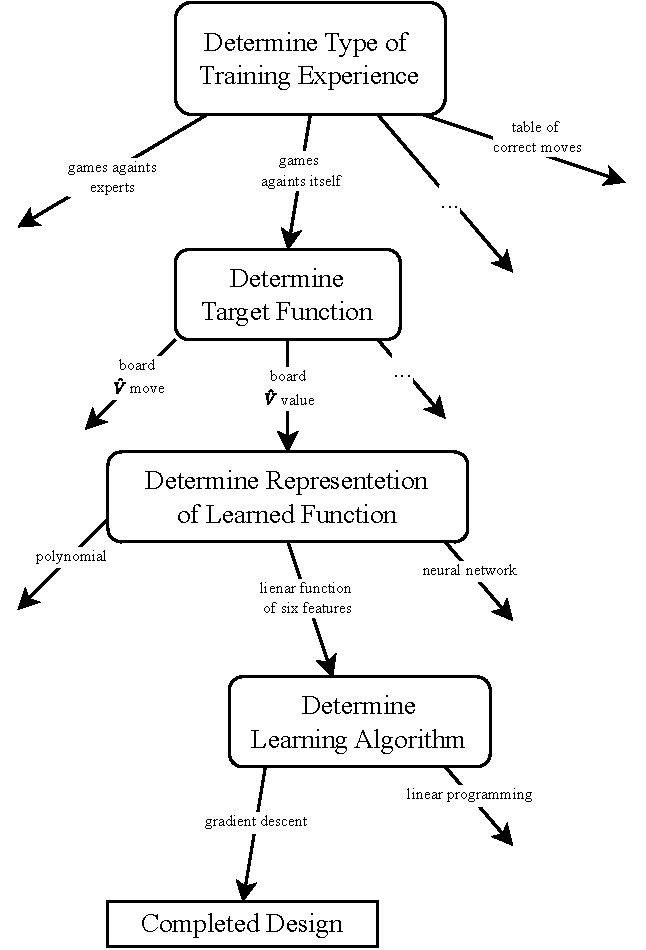
\includegraphics[width=0.35\textwidth]{images/DesignChoice.pdf}
	\caption{Design Choices}
	\label{img:DesignChoice}
\end{figure}

\newpage
\section{Types of Machine Learning Problems}

Machine learning is a vast field encompassing a variety of problem types, each defined by the kind of data available and the way the model learns from it.
Broadly speaking, learning problems can be divided into three main categories:
\begin{itemize}
	\item \textbf{Supervised Learning}
	\item \textbf{Unsupervised Learning}
	\item \textbf{Reinforcement Learning}
\end{itemize}

Each of these paradigms addresses different situations and goals. In what follows we provide an overview to clarify their purposes and fundamental differences.

\bigskip
\textbf{Supervised Learning.}
In supervised learning, the model is trained on a dataset that contains \emph{input–output pairs}.
Each example is composed of an input vector $x$ (the features) and a corresponding label or target value $y$.
The goal is to learn a mapping $f: X \rightarrow Y$ such that, given a new unseen input $x'$, the model can predict its output $\hat y = f(x')$ as accurately as possible.

The term ``supervised'' refers to the fact that the learning process is guided by known answers: the model is explicitly told what the correct output should be for each example.
The performance of the model is typically measured by comparing its predictions $\hat y$ with the true labels $y$ through a loss function.

Supervised learning problems are commonly divided into two subcategories:
\begin{itemize}
	\item \textbf{Classification:} the goal is to assign each input to one of a finite set of categories.
	      Examples include recognizing handwritten digits, detecting spam emails, or classifying medical images into healthy and pathological classes.
	\item \textbf{Regression:} the goal is to predict a continuous value rather than a discrete label.
	      Typical examples are forecasting house prices, estimating temperature, or predicting stock market trends.
\end{itemize}

Supervised learning is the most widely studied and applied paradigm, as labeled data are often available and the learning objectives are clearly defined.

\bigskip
\textbf{Unsupervised Learning.}
In contrast to supervised learning, in unsupervised learning we do \emph{not} have labeled data.
The dataset consists only of input examples $\{x_1, x_2, \dots, x_n\}$ without corresponding outputs.
The aim is to uncover hidden structures or patterns within the data itself.

Since there is no external notion of ``correctness,'' the model must learn to organize or represent the data based solely on its internal relationships.
Typical unsupervised tasks include:
\begin{itemize}
	\item \textbf{Clustering:} grouping similar data points together according to some notion of similarity or distance (e.g., grouping customers by purchasing behavior or documents by topic).
	\item \textbf{Dimensionality Reduction:} discovering compact representations of high-dimensional data while preserving essential information (e.g., using Principal Component Analysis or autoencoders to visualize complex data in two dimensions).
\end{itemize}

Unsupervised learning is often used for data exploration, feature extraction, or as a preprocessing step for supervised tasks.

\bigskip
\textbf{Reinforcement Learning.}
Reinforcement learning (RL) represents a distinct paradigm where an \emph{agent} learns by interacting with an \emph{environment}.
At each time step, the agent observes the current state $s$, selects an action $a$, and receives a numerical \emph{reward} $r$ that measures the immediate outcome of that action.
Over time, the agent aims to learn a policy $\pi(s)$ that maximizes the expected cumulative reward.

Unlike supervised learning, there are no fixed ``correct'' outputs to imitate.
Instead, the agent must discover good strategies through \emph{trial and error}, balancing exploration of new actions and exploitation of known rewarding ones.

Reinforcement learning is widely used in scenarios where decisions must be made sequentially and outcomes depend on long-term consequences—for example, game playing (such as chess or Go), robotics control, and autonomous driving.

\bigskip
\begin{figure}[h!]
	\centering
	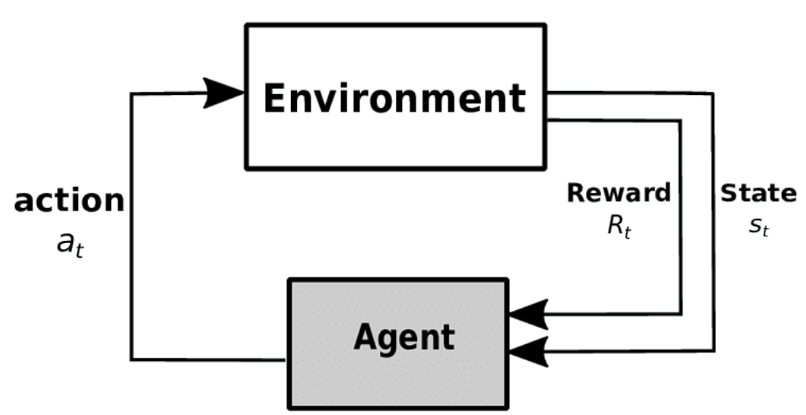
\includegraphics[width=0.35\textwidth]{images/RL_diagram.png}
	\caption{Reinforcement Learning}
	\label{img:ReinforcementLearning}
\end{figure}

\bigskip
In summary, these three paradigms differ in how they use data:
supervised learning learns from labeled examples, unsupervised learning seeks patterns in unlabeled data, and reinforcement learning learns through interaction and feedback from the environment.
Together, they form the conceptual foundation for the majority of modern machine learning systems.

\begin{definition}
	Given a function $f: X \rightarrow Y$, and a training set $X_D \subset X$ containing information about $f$, \textbf{learning} the function $f$ means computing an approximated function $\hat f$ such that it is as close as possible to $f$ on $X$:
	\begin{equation}
		\hat f(x) \simeq f(x), \quad x \in X.
	\end{equation}
\end{definition}

This is a challenging problem because the true function $f$ is unknown and usually not computable, while the input space $X$ is often extremely large or continuous.
In practice, we can only access a small subset $X_D$, so $\hat f$ must be learned from limited examples and still perform well on unseen data — this property is known as \textbf{generalization}.\bigskip

The goal of learning is therefore to find, within a chosen family of models, the function $\hat f$ that best approximates $f$ on the training set and generalizes to new inputs.
This balance between fitting known data and adapting to new situations is the core difficulty of every machine learning problem.\bigskip

Machine learning problems can be classified in terms of the input data set $D$, given a target function $f:X\rightarrow Y$ a problem is\begin{itemize}
	\item a \textbf{supervised learning} problem if the dataset is labeled: $D=\bigcup_{i=1}^n\{(x_i,y_i)\}\subset X\times Y$ .
	\item an \textbf{unsupervised learning} problem if the dataset is not labeled: $D=\bigcup_{i=1}^n\{(x_i)\}\subset X$.
	\item a \textbf{reinforcement learning} problem, the condition on the input dataset will be discussed later.
\end{itemize}

The problems can also be classified in terms of the target function $f : X \rightarrow Y$, that is, according to the type of input space $X$ and output space $Y$.
Different combinations of these sets define different learning settings:
\begin{align*}
	 & X=\begin{cases}
		     A_1\times \dots \times A_m, \ A_i \text{ finite set} \ \ \textbf{(Finite Discrete Problem)} \\
		     \R^n \ \ \textbf{(Continuous)}
	     \end{cases} \\
	 & Y=\begin{cases}
		     \R^k \ \ \textbf{(Regression)} \\
		     \{C_1,C_2\times C_k\} \ \ \textbf{(Classification)}
	     \end{cases}
\end{align*}

Here, $X$ represents the \textbf{input space}, that is, the domain of possible observations or feature vectors, while $Y$ represents the \textbf{output space}, the type of value the model aims to predict.

\begin{itemize}
	\item In a \textbf{regression problem}, the goal is to predict one or more real-valued quantities, such as temperature, price, or time. The function $f$ is thus continuous, mapping inputs in $\R^n$ to outputs in $\R^k$.
	\item In a \textbf{classification problem}, the goal is to assign each input to one of a finite number of categories (classes) $\{C_1, \dots, C_k\}$, such as recognizing digits, detecting spam, or identifying an animal in an image.
\end{itemize}

\newpage
Here we offer two examples of, respectevely, regression and classification problems:

\bigskip
\begin{figure}[h!]
	\centering
	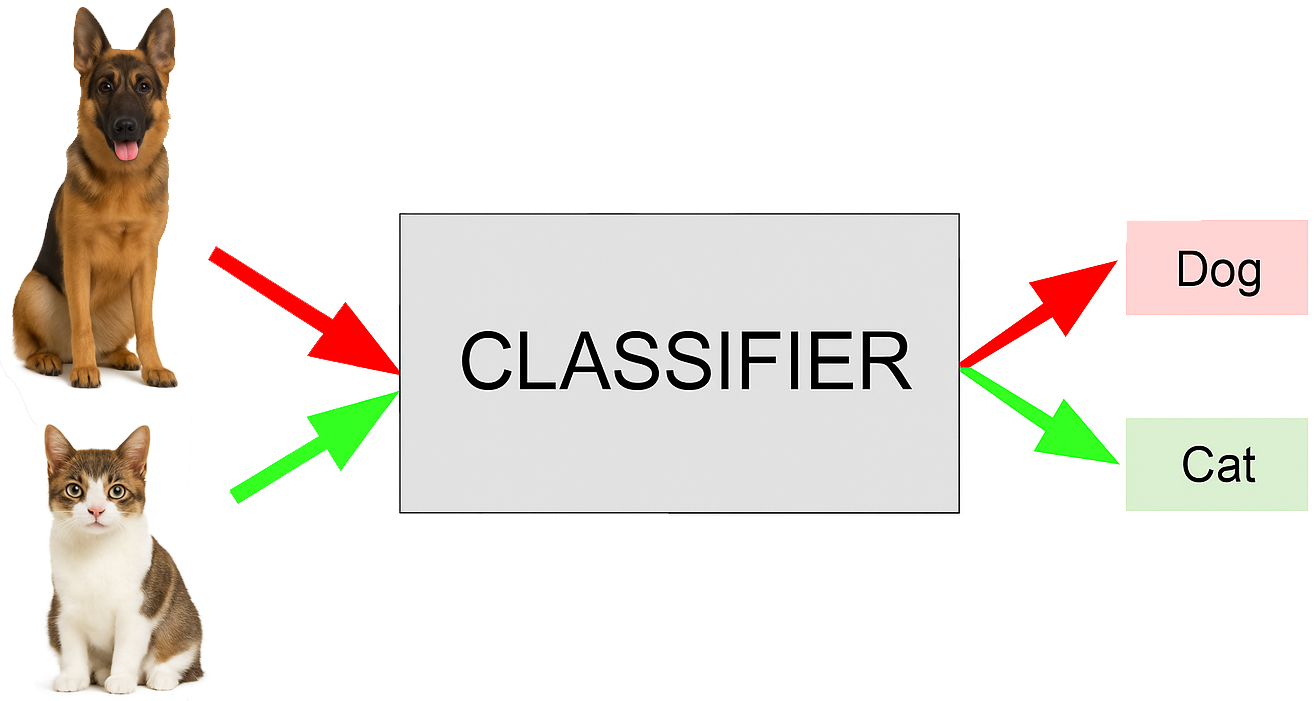
\includegraphics[width=0.35\textwidth]{images/classifier.png}
	\caption{A Classification Problem}
	\label{img:ClassificationProblem}
\end{figure}

\bigskip
\begin{figure}[h!]
	\centering
	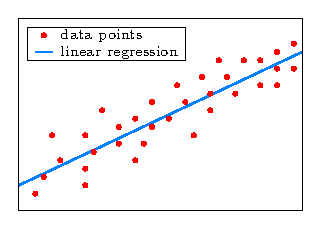
\includegraphics[width=0.35\textwidth]{images/regression.eps}
	\caption{A Regression Problem}
	\label{img:RegressionProblem}
\end{figure}

\bigskip
A useful \textit{special case} is known as \textbf{concept learning}, where both input and output spaces are discrete:
\begin{align*}
	 & X = A_1\times \dots \times A_m, \ A_i \text{ finite set} \\
	 & Y = \{0,1\}
\end{align*}

In concept learning, the output consists in only two classes, the target function $c:X\rightarrow\{0,1\}$ maps any kind of input in one of two distinct values. The following example model a program that predict if is a good day to play Tennis, the input set is $$
	X=Day\times Outlook \times Temperature \times Humidity \times Wind
$$
the output set is $PlayTennis=\{\text{Yes, No}\}$. An example of data samples:\begin{center}
	\begin{tabular}{cccccc}
		\toprule
		$Day$ & $Outlook$ & $Temperature$ & $Humidity$ & $Wind$ & $PlayTennis$ \\
		\midrule
		D1    & Sunny     & Hot           & High       & Weak   & No           \\
		D2    & Sunny     & Hot           & High       & Strong & No           \\
		D3    & Overcast  & Hot           & High       & Weak   & Yes          \\
		D4    & Rain      & Mild          & High       & Weak   & Yes          \\
		D5    & Rain      & Cool          & Normal     & Weak   & Yes          \\
		D6    & Rain      & Cool          & Normal     & Strong & No           \\
		D7    & Overcast  & Cool          & Normal     & Strong & Yes          \\
		D8    & Sunny     & Mild          & High       & Weak   & No           \\
		D9    & Sunny     & Cool          & Normal     & Weak   & Yes          \\
		D10   & Rain      & Mild          & Normal     & Weak   & Yes          \\
		D11   & Sunny     & Mild          & Normal     & Strong & Yes          \\
		D12   & Overcast  & Mild          & High       & Strong & Yes          \\
		D13   & Overcast  & Hot           & Normal     & Weak   & Yes          \\
		D14   & Rain      & Mild          & High       & Strong & No           \\
		\bottomrule
	\end{tabular}
\end{center}

\newpage
\bigskip
Finally, classification problems are often referred to as \textit{pattern recognition problems},
since their purpose is to identify the category or pattern to which a specific instance belongs.

\bigskip
Some examples are:\begin{itemize}
	\item Face/Object/Character Recognition
	\item Speech/Sound Recognition
	\item Medical Diagnosis
	\item Document Classification.
\end{itemize}

\bigskip
\section{Performance Evaluation}

Usually, we call \textbf{Hypothesis} a possible learned function $h$, and we define $H$ as the \textbf{Hypothesis space}, such space contains all possible function that can be learnt (all possible approximation of the target function). In this terms, a \textbf{learning problem} is described as a search in the hypothesis space using the given dataset $D$, that aims to find the best possible approximation $h^*$:

\begin{equation}\label{sol_hypothesis}
	h^*=\arg \max_{h\in H} Performance(h,D)
\end{equation}

\bigskip
\begin{figure}[h!]
	\centering
	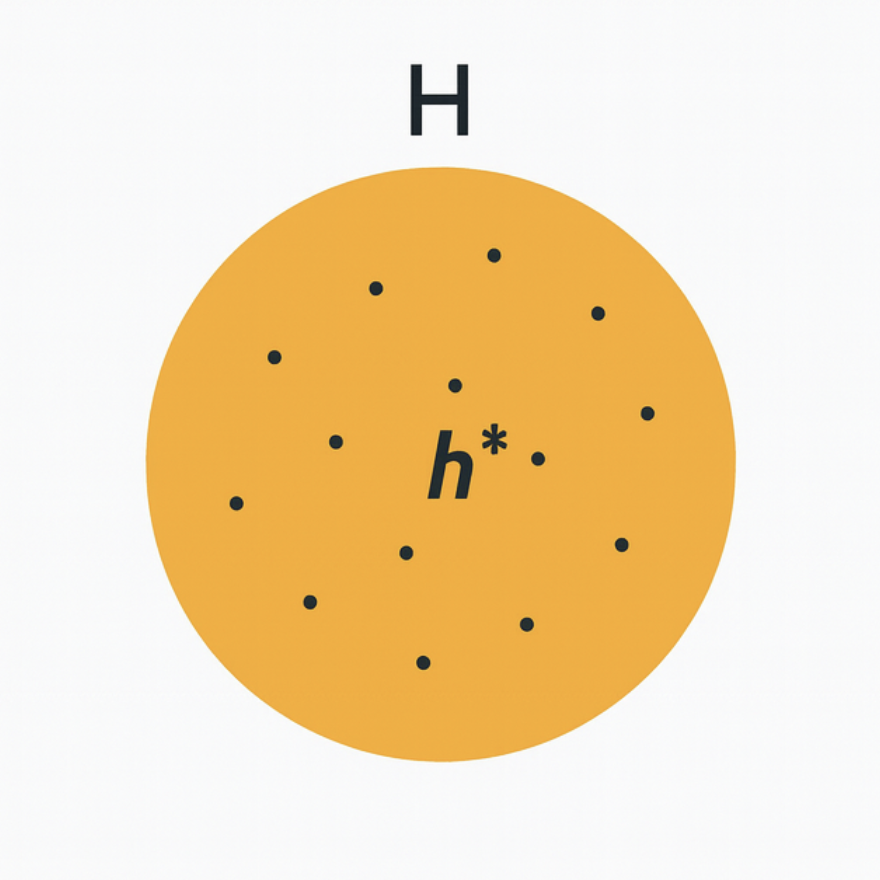
\includegraphics[width=0.35\textwidth]{images/HypotesisSpace.png}
	\caption{An Hypothesis in the Hypothesis Space}
	\label{img:HypothesisSpace}
\end{figure}

\subsection{Concept Learning}

We now focus on \textbf{concept learning}, which corresponds to the special case of binary classification.

\bigskip
Let the target function be
\begin{equation}
	c : X \rightarrow \{0,1\}.
\end{equation}

We are given a dataset
\begin{equation}
	D = \bigcup_{i=1}^{n} \{(x_i, c(x_i))\},
\end{equation}
where each example $(x_i, c(x_i))$ pairs an input $x_i \in X$ with its corresponding label $c(x_i)$, as defined by the unknown concept $c$. We denote by $X_D$ the set of input points that appear in the dataset.

\bigskip
In an ideal scenario, all training examples are labeled correctly — we call such a dataset \textbf{noise-free} or \textbf{perfect}:
\[
	D_{\text{perfect}} = \bigcup_{i=1}^n \{(x_i, c(x_i))\}.
\]

However, in practice data are often affected by \textbf{noise}, meaning that some labels or features may be incorrect, uncertain, or perturbed by random variation. We can represent this as:
\[
	D_{\text{noisy}} = \bigcup_{i=1}^n \{(x_i, c(x_i) + \varepsilon_i)\}, \qquad \varepsilon_i \in \mathbb{R}.
\]

Here, $\varepsilon_i$ represents the \textbf{noise term}, which can arise from measurement errors, subjective labeling, missing information, or inherent randomness in the process that generated the data. Noise introduces ambiguity because the same input $x_i$ might be associated with inconsistent labels in different samples.

\bigskip
\begin{definition}
	Given a target function $c$ and a set of sample points $X_D$, a hypothesis $h$ is said to be \textbf{consistent} with the training data if
	\[
		h(x) = c(x), \quad \forall x \in X_D.
	\]
\end{definition}

In other words, a consistent hypothesis correctly classifies all examples in the training dataset.
When the dataset is noise-free, it is usually possible to find one or more consistent hypotheses within $H$.
However, in the presence of noise, perfect consistency may be impossible — in such cases, learning algorithms aim to find the \emph{most consistent} or \emph{best-fitting} hypothesis, minimizing the number of classification errors rather than eliminating them entirely.

\bigskip
The \textbf{Version Space} $VS_{H,D}$ is the set of all consistent hypothesis:\begin{equation}
	VS_{H,D}=\{h \ : \ h(x)=c(x), \ \ \forall x\in X_D\}\subset H.
\end{equation}
A solution that does not lie in the version space is probably not a good solution.\bigskip

\bigskip
\begin{figure}[h!]
	\centering
	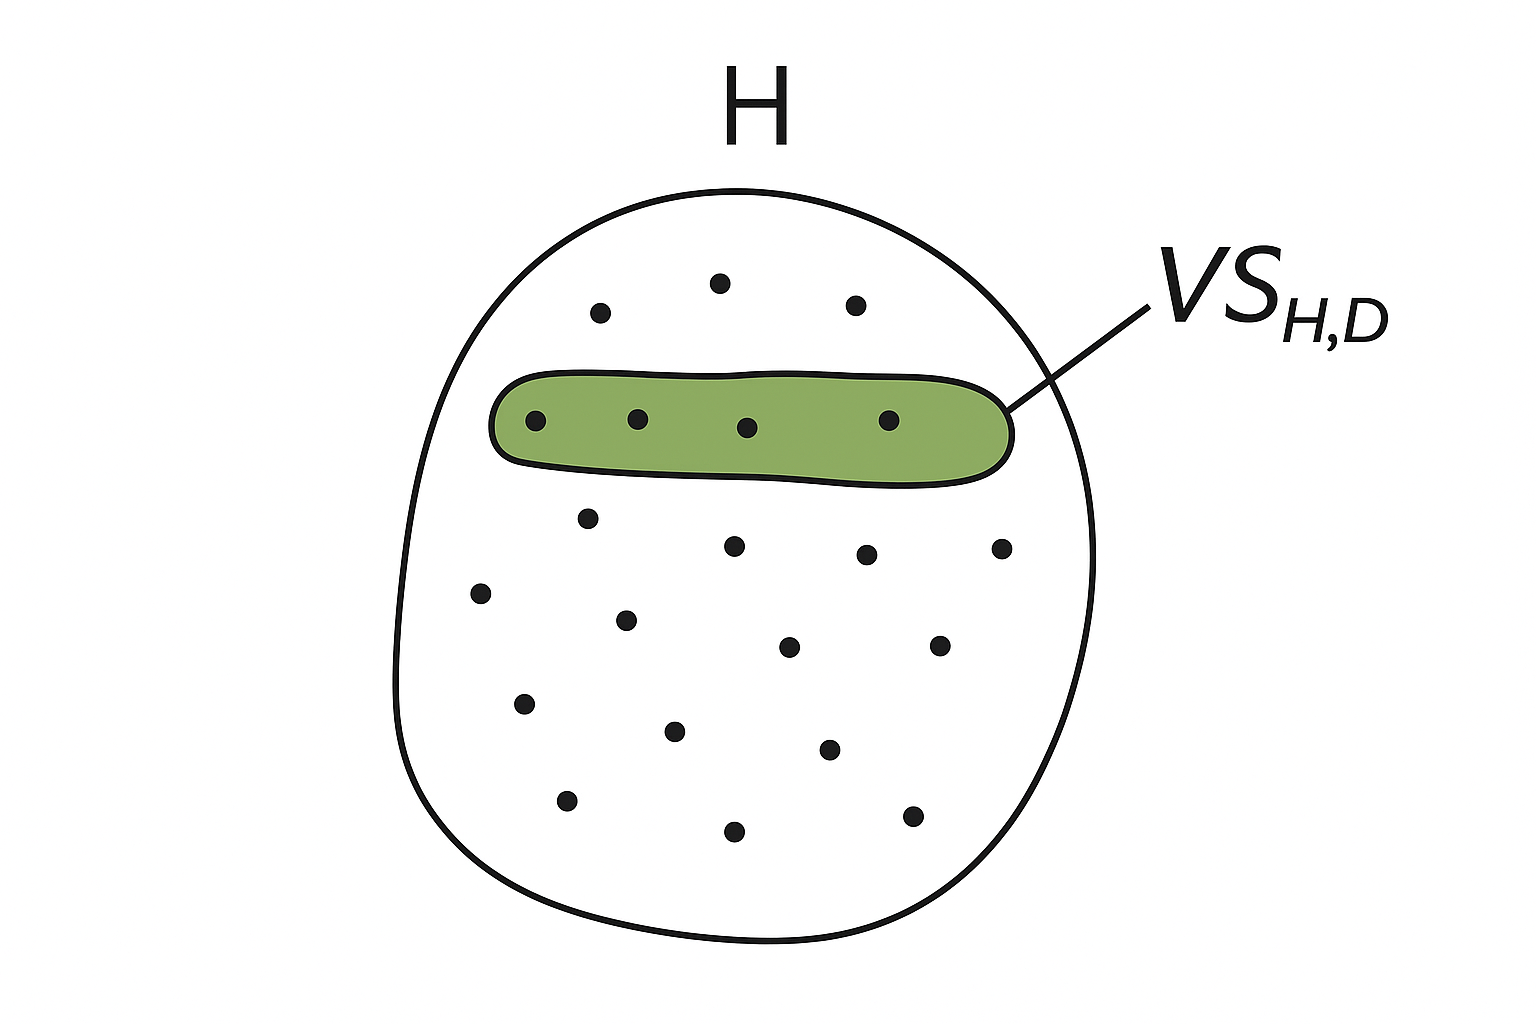
\includegraphics[width=0.35\textwidth]{images/VersionSpace.png}
	\caption{A Version Space in the Hypothesis Space}
	\label{img:VersionSpace}
\end{figure}

\subsection{Overfitting and Underfitting}

Let's consider an example. Let $c$ be the following target function:
\begin{equation}
	c:\N\rightarrow\{-,+\}.
\end{equation}
The dataset is given by:
\begin{equation}
	D=\{(1,+),(3,+),(5,+),(6,-),(8,-),(10,-)\}.
\end{equation}

Given a hypothesis space $H$, consider the following four hypotheses:
\begin{align*}
	 & h_1(n)=+\iff n\text{ is odd},               \\
	 & h_2(n)=+\iff n\le 5,                        \\
	 & h_3(n)=+\iff n\text{ is either 1 or prime}, \\
	 & h_4(n)=+\iff n\in\{1,3,5\}.
\end{align*}

If $n=11$, then:
\begin{align*}
	 & h_1(11)=+, \\
	 & h_2(11)=-, \\
	 & h_3(11)=+, \\
	 & h_4(11)=-.
\end{align*}

The problem is that we cannot tell which of the four hypotheses is “better.”
They all fit the training data equally well, but they generalize differently on unseen examples.

\bigskip
Now, consider an expanded hypothesis space $H'$, defined as the power set of $H$:
\begin{equation}
	H'=\mathcal P(H)=\{I \mid I\subseteq H\}.
\end{equation}
The set $H'$ contains more information than $H$. For $\theta \in H'$, we define:
\begin{align}
	\theta    & = \bigcup_i\{h_i\},                     \\
	\theta(x) & =\operatorname{maj}\bigcup_i\{h_i(x)\},
\end{align}
where the function $\operatorname{maj}$ returns the most frequent label in the set.
If two labels occur with the same frequency, $\operatorname{maj}$ is undefined.

\bigskip
For instance, at $n=11$:
\begin{equation}
	\theta(11)=\operatorname{maj}\{h_1(11),h_2(11),h_3(11),h_4(11)\}=\operatorname{maj}\{+,-,+,-\},
\end{equation}
so the classification is undefined.

\bigskip
This means that even though $H'$ is more expressive than $H$, it fails to generalize: it cannot classify a point that $H$ could classify.
This situation is known as \textbf{overfitting}: the hypothesis space is too rich, leading to instability and poor generalization.

\bigskip
Now consider another target function:
\begin{equation}
	c:\N^2\rightarrow\{+,-\},
\end{equation}
with a dataset $D$ plotted on a 2D plane:

\begin{center}
	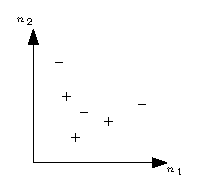
\includegraphics[width=0.25\textwidth]{images/N2_hypothesis_1.eps}
\end{center}

Let $H$ be the set of functions that assign the label $+$ to all points within a rectangle $R$ and $-$ otherwise:
\begin{equation}
	h\in H \iff \Big( \exists R=\{(x,y): a\le x\le b,\ c\le y\le d\} \text{ such that } h(x,y)=+ \iff (x,y)\in R \Big).
\end{equation}

In this case, no consistent hypothesis exists in $H$, because no single rectangle can include all $+$ points while excluding all $-$ points:

\begin{center}
	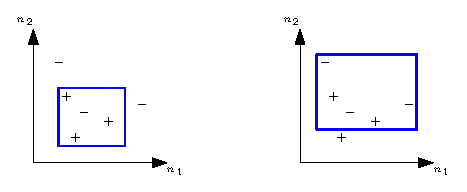
\includegraphics[width=0.6\textwidth]{images/N2_hypothesis_2.eps}
\end{center}

If we extend the hypothesis space to $H'=\mathcal P(H)$, we can represent a function using multiple rectangles.
Now consistent hypotheses exist, but the model becomes too specific and fails to generalize — predicting $+$ almost everywhere:

\begin{center}
	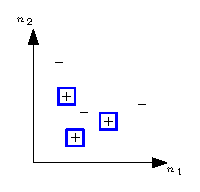
\includegraphics[width=0.25\textwidth]{images/N2_hypothesis_3.eps}
\end{center}

This illustrates the trade-off between model complexity and generalization ability:
\begin{itemize}
	\item A \textbf{too simple} hypothesis space cannot capture the true concept (\textbf{underfitting});
	\item A \textbf{too complex} hypothesis space fits the training data perfectly but fails to generalize (\textbf{overfitting}).
\end{itemize}

\bigskip
If $n$ measures the “size” or expressive power of the hypothesis space, we can observe the following trend in model performance:

\begin{figure}[h!]
	\centering
	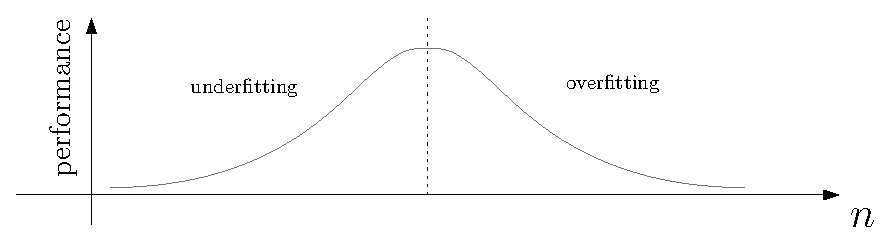
\includegraphics[width=0.65\textwidth]{images/fitting.eps}
	\caption{The trade-off between underfitting and overfitting.}
	\label{img:fitting_trend}
\end{figure}

As model complexity increases, training error decreases, but test error eventually rises after a certain point — showing that the best hypothesis is not the most complex one, but the one that achieves the right balance between fit and generalization.

\bigskip
\subsection{Error Estimation and Performance Metrics}

When we train a machine learning model, we want to evaluate how good a hypothesis $h$ is compared to others — not only on the training data, but also on unseen examples.
Since the available dataset represents only a small sample of all possible inputs, this evaluation cannot be done deterministically.
We therefore rely on \textbf{statistical methods} to estimate the model’s true performance.

\bigskip
Let us consider a target function
\begin{equation}
	f : X \rightarrow Y,
\end{equation}
where $Y$ is countable (classification problem).
We assume that examples are drawn according to an unknown probability distribution $\mathcal D$ over the input space $X$.

\begin{definition}\label{def:prob_distr}
	If $X$ is a countable subset of $\R^n$, $\mathcal D$ is a probability distribution on $X$ if
	\begin{eqnarray}
		\forall x\in X, \ \ \mathcal D(x)\in [0,1],
	\end{eqnarray}
	and
	\begin{align*}
		\sum_{x\in X}\mathcal D(x)=1.
	\end{align*}
	\newpage
	If $X$ is an uncountable subset of $\R^n$, $\mathcal D$ is a probability distribution on $X$ if
	\begin{eqnarray}
		\forall x\in X, \ \ \mathcal D(x)\ge 0,
	\end{eqnarray}
	and
	\begin{align*}
		\int_X\mathcal D(x)\,dx=1.
	\end{align*}
\end{definition}

The distribution $\mathcal D$ represents the underlying process that generates the data.
Since it is unknown, we can only estimate a model’s performance statistically — using finite samples from $\mathcal D$.

\bigskip
\begin{definition}
	Given a target function $f:X\rightarrow Y$, an hypothesis $h$ and a probability distribution $\mathcal D$ on $X$, the \textbf{true error} is the probability that $h$ will misclassify an instance $x\in X$ drawn according to the distribution $\mathcal D$:
\end{definition}
\begin{equation}
	\text{error}_{\mathcal D}(h)=
	\Prob_{x\sim \mathcal D}
	(f(x)\ne h(x))
\end{equation}
\textbf{Note}: With $x\sim \mathcal D$, we mean that $x$ was extracted from $X$ according to the probability distribution $\mathcal D$. We remind that, if $\mathcal D(x)=p$, then, the probability of extracting $x$ from $X$ by taking a random element is $p$.\bigskip

Since we can't compute $f$ for all $x\in X$, the true error can't be computed. We need to define an estimation of the error given by the sample set extracted from $X$.
\begin{definition}
	Given a target function $f:X\rightarrow Y$, an hypothesis $h$ and a sample (finite) set $\mathcal S\subset X$, the  \textbf{sample error} is defined as follows:
\end{definition}\begin{equation}
	\text{error}_{\mathcal S}(h)=
	\frac{1}{|\mathcal S|}\sum_{x\in\mathcal S}\delta(f(x)\ne h(x))
\end{equation}
where\begin{itemize}
	\item $\delta(\phi)=1$ if $\phi$ is true
	\item $\delta(\phi)=0$ if $\phi$ is false.
\end{itemize}
The sample error can be computed since, for each $x\in\mathcal S$, we know the value of $f(x)$. Is an approximation of the true error that depends from the sample set $\mathcal S$.\bigskip

Since $\text{error}_{\mathcal S}(h)$ depends from the choice of $\mathcal S$, is not fixed, but we can model it as a random process, by extracting $n$ random values from $X$ according to the distribution $\mathcal D$ to construct $\mathcal S$, and we can evaluate the expected value of $\text{error}_{\mathcal S}(h)$ denoted \begin{equation}
	\VA(\text{error}_{\mathcal S}(h)).
\end{equation}
We want to formalize this expected value, in this case the sample error is a random variable that assign to each subset $\mathcal S$ of $X$ of size $n$ a number between 0 and $1$:
\begin{align}
	 & \text{error}_{\mathcal S}(h) : \Omega \rightarrow [0,1]                \\
	 & \Omega =\{\mathcal S \ : \ \mathcal S \subset X \land |\mathcal S|=n\}
\end{align}
in this context, $n$ is fixed. The probability of getting a certain value $\gamma$ from this random variable, is the probability to extract from $X$ a subset $\mathcal S$ of $n$ items such that, the sample error is $\gamma$, and this depends from the probability distribution $\mathcal D$ on $X$. The expected value $\VA(\text{error}_{\mathcal S}(h))$ is now well defined.

\newpage
\subsection{Unbiased Estimation}

\begin{definition}
	The \textbf{bias} is defined as the expected difference between the sample error and the true error:
\end{definition}
\begin{equation}
	\VA(\text{error}_{\mathcal S}(h)) - \text{error}_{\mathcal D}(h).
\end{equation}

An estimator is said to be \textbf{unbiased} if its expected value equals the quantity it aims to estimate, that is:
\begin{equation}
	\text{bias} = 0 \ \ \implies \ \ \VA(\text{error}_{\mathcal S}(h)) = \text{error}_{\mathcal D}(h).
\end{equation}

\bigskip
If we compute the sample error on the same data used to train the hypothesis $h$, the resulting estimate is typically \emph{optimistically biased} — the model performs better on familiar examples than on unseen ones.
To obtain an unbiased estimate of the true error, we must evaluate $h$ on data that were not used during training.

\bigskip
Let $D$ be the available dataset. We split it into two disjoint subsets:
\begin{align}
	 & D = T \cup S,         \\
	 & T \cap S = \emptyset,
\end{align}
where $T$ (the \textbf{training set}) is used to learn the hypothesis $h$, and $S$ (the \textbf{test set}) is used to estimate its performance.
Typically, $\frac{|T|}{|D|} \simeq \frac{2}{3}$.

\bigskip
The sample error is then computed as:
\begin{equation}
	\text{error}_{S}(h) = \frac{1}{|S|}\sum_{x \in S} \delta(f(x) \ne h(x)).
\end{equation}

It is ideal to choose $T$ and $S$ such that they are drawn from the same underlying distribution over the features.
In that case, the random variable $\text{error}_{S}(h)$ is an \textbf{unbiased estimator} of the true error $\text{error}_{\mathcal D}(h)$.

\bigskip
\subsection{The Cross Validation Algorithm and Other Performance Metrics}

Estimating a model’s true error from limited data can be unreliable, since a single train–test split may depend heavily on which samples are chosen.
To obtain a more stable and statistically sound estimate, we can use \textbf{cross-validation}, which averages results over multiple train/test partitions.

\bigskip
The following algorithm estimates the expected value of the sample error.
The larger the dataset $D$, the more accurate this estimation will be.
Let $L$ denote a fixed learning algorithm and let $h = L(T)$ be the hypothesis learned from a training set $T$.

\begin{algorithm}
	\caption{K-Fold Cross Validation}\label{alg:CrossVal}
	\begin{algorithmic}
		\Require $D$, $k$, $h$, $L$
		\State partition $D$ into $k$ disjoint subsets $S_1, S_2, \dots, S_k$
		\For{$i=1,2,\dots,k$}
		\State $T_i \leftarrow D \setminus S_i$
		\State $h_i \leftarrow L(T_i)$
		\State $\delta_i = \text{error}_{S_i}(h_i)$
		\EndFor
		\State\Return $\text{error}_{L,D} = \displaystyle\frac{1}{k}\sum_{i=1}^{k}\delta_i$
	\end{algorithmic}
\end{algorithm}

In this procedure, each subset $S_i$ serves once as a test set while the remaining $k-1$ subsets form the training data.
The final estimate of the model error is the average of the $k$ test errors, providing a more robust measure of generalization than a single holdout split.

\bigskip
We define the accuracy of a learning algorithm $L$ as
\begin{equation}
	\text{accuracy} = 1 - \text{error}_{L,D}.
\end{equation}
Cross-validation can also be used to compare two learning algorithms, $L_a$ and $L_b$, by evaluating the difference in their cross-validated errors, as shown in Algorithm~\ref{alg:CrossVal_compare}.

\begin{algorithm}
	\caption{Accuracy Comparator}\label{alg:CrossVal_compare}
	\begin{algorithmic}
		\Require $D$, $k$, $L_a$, $L_b$
		\State partition $D$ into $k$ disjoint subsets $S_1,S_2,\dots,S_k$
		\For{$i=1,2,\dots,k$}
		\State $T_i \leftarrow D \setminus S_i$
		\State $h_a \leftarrow L_a(T_i)$
		\State $h_b \leftarrow L_b(T_i)$
		\State $\delta_i = \text{error}_{S_i}(h_a) - \text{error}_{S_i}(h_b)$
		\EndFor
		\State\Return $\bar{\delta} = \displaystyle\frac{1}{k}\sum_{i=1}^k \delta_i$
	\end{algorithmic}
\end{algorithm}

A positive value of $\bar{\delta}$ indicates that $L_b$ performs better on average, while a negative value favors $L_a$.

\bigskip
\textbf{Remarks (Optional).}
\begin{itemize}
	\item Typical values for $k$ are $5$ or $10$: smaller $k$ reduces computation, larger $k$ reduces variance.
	\item The special case $k = |D|$ corresponds to \textbf{leave-one-out cross-validation (LOOCV)}.
	\item When class proportions must be preserved across folds, we use \textbf{stratified cross-validation}.
\end{itemize}

\bigskip
Now that we defined the sample error, we can give a formal definition of overfitting. Let $h$  to be an hypothesis for a model, $h$ is overfitting is exists an hypothesis $h'$ such that\begin{align}
	 & \text{error}_{S}(h)<\text{error}_{S}(h')                   \\ &\land\\
	 & \text{error}_{\mathcal D}(h)>\text{error}_{\mathcal D}(h')
\end{align}

Let's consider other performance metrics in binary classification. Let $f:X\rightarrow\{-,+\}$ to be the target function ad let $D$ to be a sample set such that, $90\%$ of elements in $D$ is of class $+$. An hypothesis that always returns $+$ will have an accuracy of $90\%$, in this scenario the dataset is \textbf{unbalanced}, so the accuracy is not a good performance metric for the model. We can consider a table that counts the number of points in the sample set that are well classified or misclassified by an hypothesis:
\begin{center}
	\begin{tabular}{c|cc|}
		\cline{2-3}
		                                 & \multicolumn{2}{c|}{predicted class}                  \\ \hline
		\multicolumn{1}{|c|}{true class} & \multicolumn{1}{c|}{+}               & -              \\ \hline
		\multicolumn{1}{|c|}{+}          & \multicolumn{1}{c|}{true positive}   & false negative \\ \hline
		\multicolumn{1}{|c|}{-}          & \multicolumn{1}{c|}{false positive}  & true negative  \\ \hline
	\end{tabular}
\end{center}
we can define two additional metrics that is useful when we deal with binary classification:\begin{itemize}
	\item the \textbf{recall} is the ability of the hypothesis to avoid false negatives and is defined as follows\begin{equation}
		      \frac{\text{true positive}}{\text{true positive}+\text{false negative}}
	      \end{equation}
	\item the \textbf{precision} is the ability of the hypothesis to avoid false positives and is defined as follows\begin{equation}
		      \frac{\text{true positive}}{\text{true positive}+\text{false positive}}
	      \end{equation}
\end{itemize}
The importance of these metrics depend on the application.

\newpage
For the classification problems we can define an extension of the previous table, called \textbf{confusion matrix}, and report how many instances of class $C_i$ are classified in class $C_j$, the main diagonal contains the accuracy for each class. An example is shown in figure \ref{img:conf_matrix}.

\bigskip
\begin{figure}[h!]
	\centering
	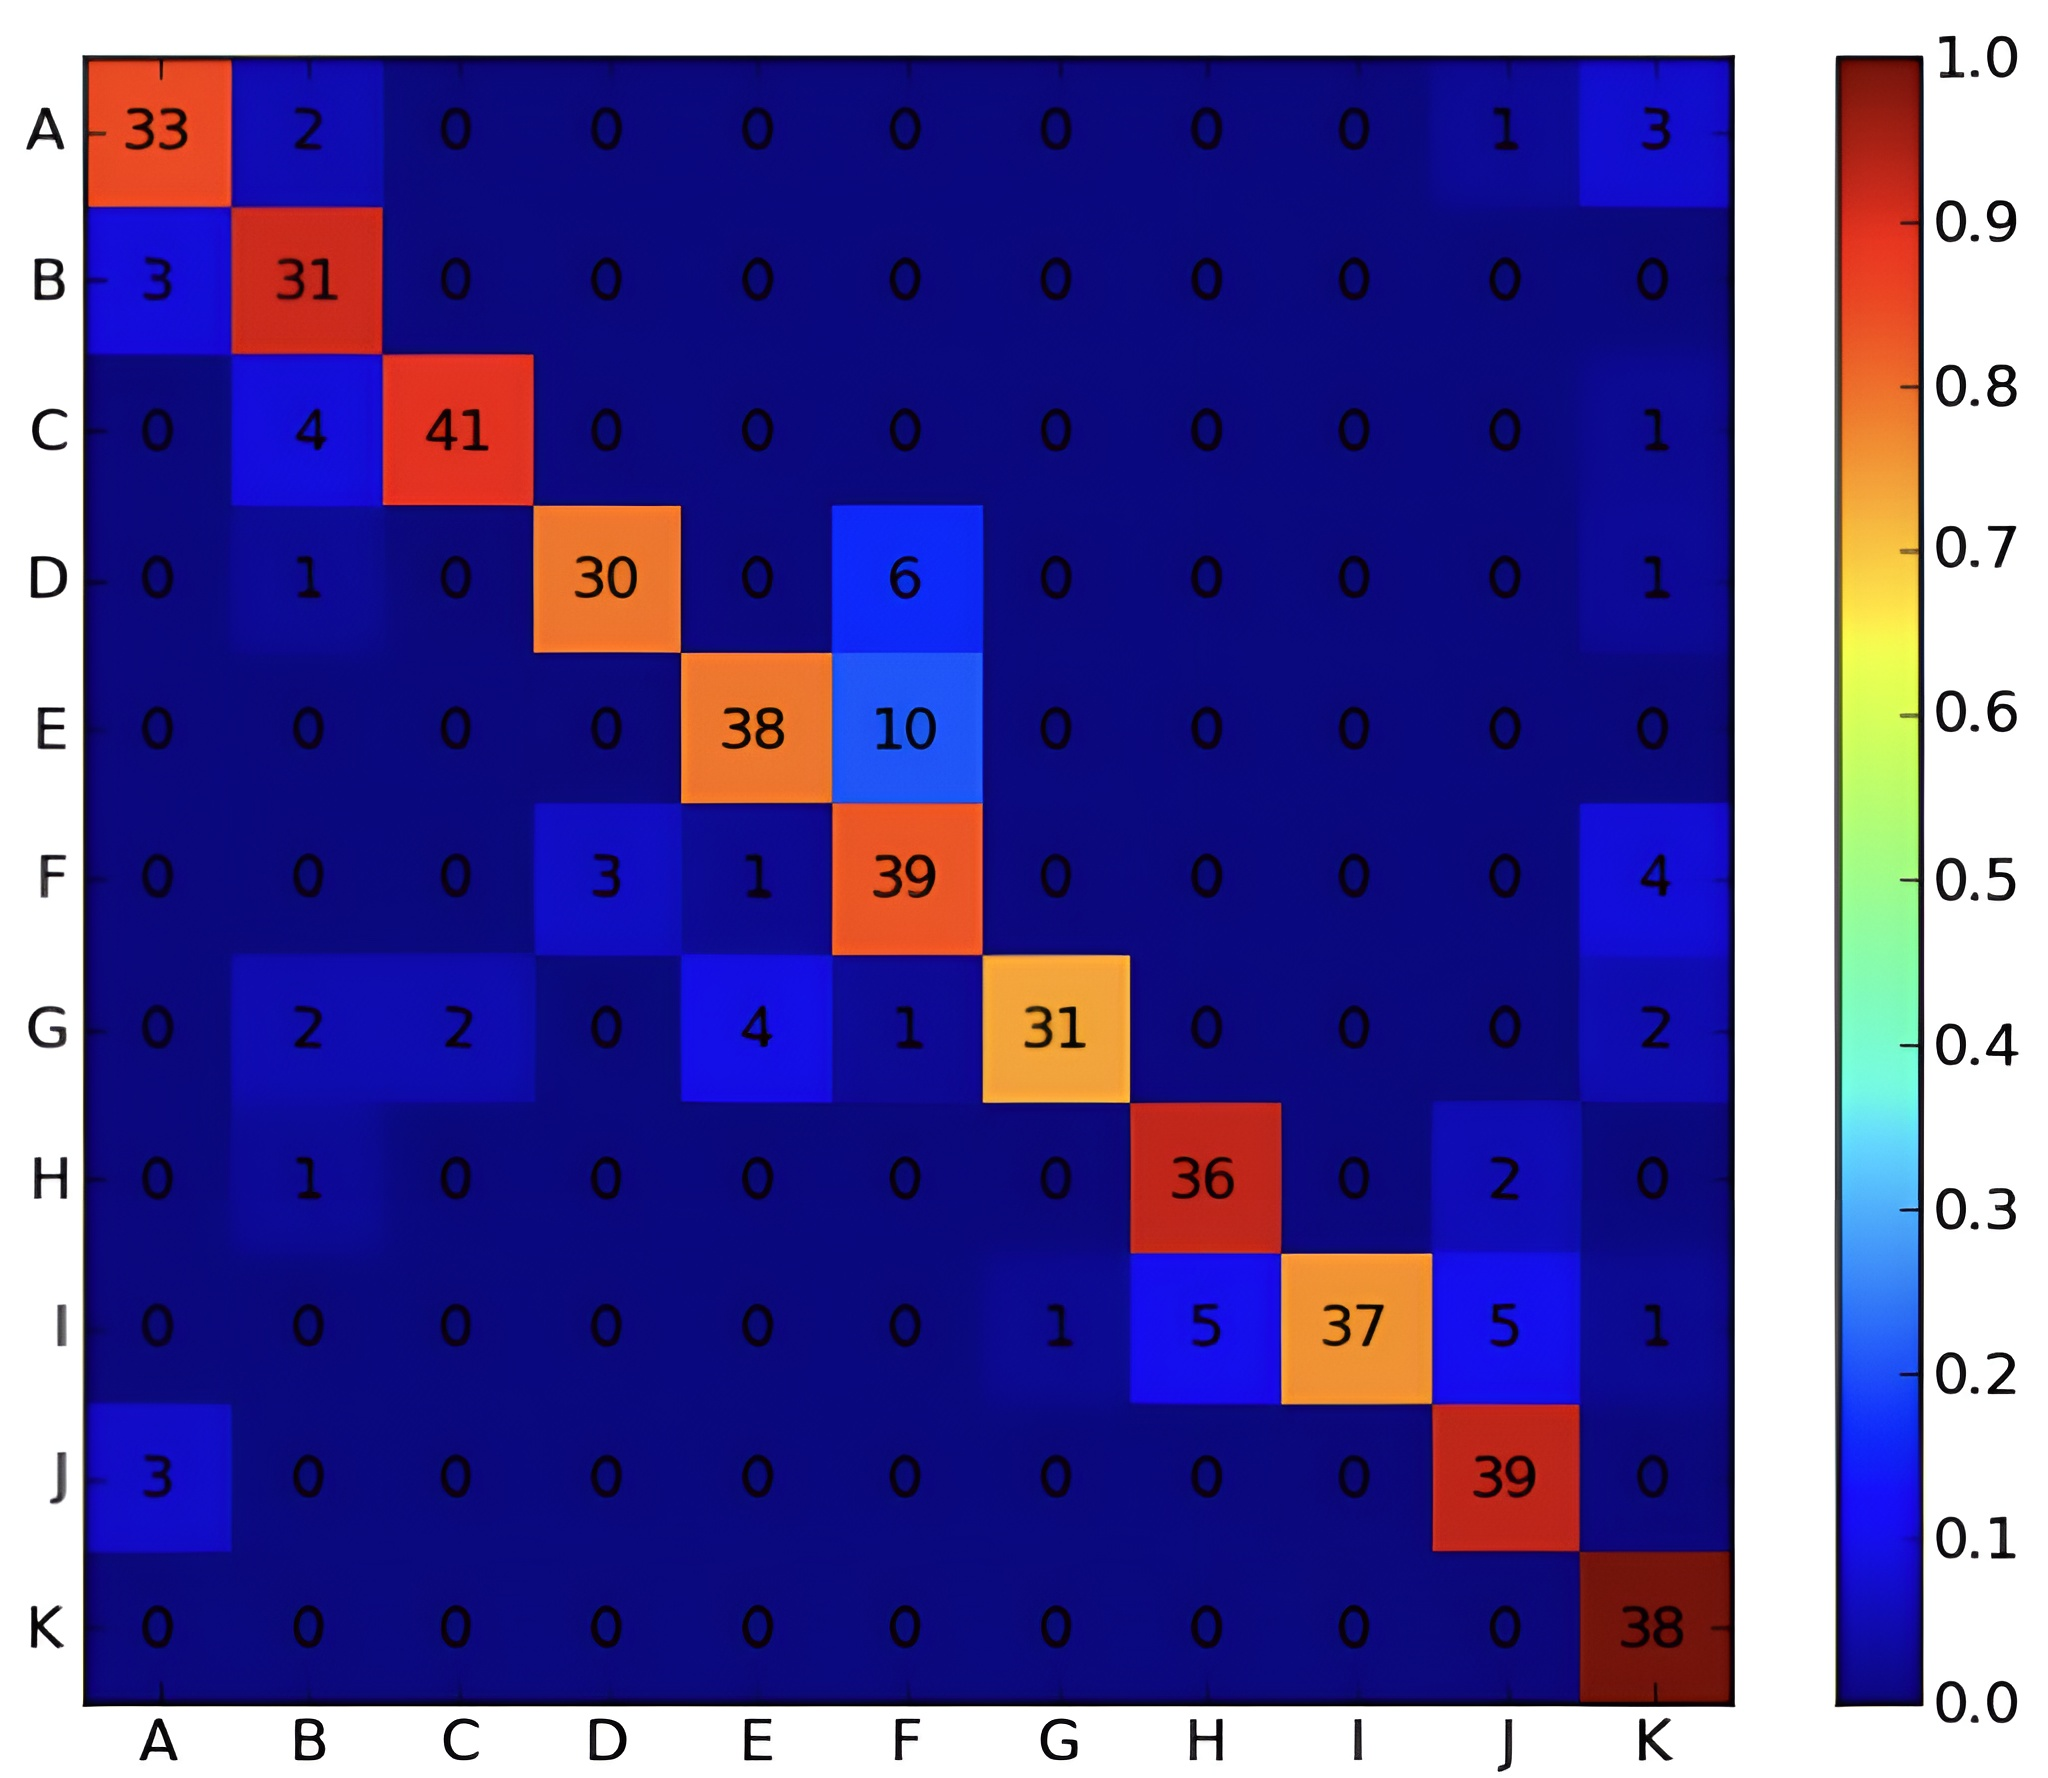
\includegraphics[width=0.3\textwidth]{images/conf_matrix.png}
	\caption{an example of a confusion matrix}
	\label{img:conf_matrix}
\end{figure}\bigskip

We consider now some performance metrics for the regression problems. Let $f:X\rightarrow\R^d$ to be the target function, and let $\hat f$ to be the learned function, for each sample $(x_i,f(x_i))$ in the dataset, we can compute the euclidian distance\begin{equation}
	|\hat f(x_i)-f(x_i)|.
\end{equation}
Let $n$ to be the number of samples, the three main metrics are the following:\begin{itemize}
	\item Mean Absolute Error\begin{equation}
		      MAE=\frac{1}{n}\sum_{i=1}^n|\hat f(x_i)-f(x_i)|
	      \end{equation}
	\item Mean Squared Error\begin{equation}
		      MSE=\frac{1}{n}\sum_{i=1}^n(\hat f(x_i)-f(x_i))^2
	      \end{equation}
	\item Root Mean Squared Error\begin{equation}
		      RMSE=\sqrt{MSE}
	      \end{equation}
\end{itemize}

The cross validation algorithm can be extended for the regression problems as shown in algorithm \ref{alg:CrossVal_regression}.

\begin{algorithm}
	\caption{K-Fold Cross Validation for Regression}\label{alg:CrossVal_regression}
	\begin{algorithmic}
		\Require $D$, $k$, $h$, $L$
		\State partition $D$ in $k$ disjoint sets $S_1,S_2\dots, S_k$
		\For{$i=1,2\dots,k$}
		\State $T_i\leftarrow  D\backslash S_i$
		\State $h_i\leftarrow L(T_i) $
		\State $\delta_i = MAE_{S_i}(h_i)$
		\EndFor
		\State\Return $\text{error}_{L,D}=\displaystyle\frac{1}{k}\sum_{i=1}^k\delta_i$
	\end{algorithmic}
\end{algorithm}

\chapter{Decision Trees}
Let's consider the following classification problem, we have a target function\begin{equation}
	c:X\rightarrow C
\end{equation}
and a data set \begin{equation}
	D=\bigcup_{i=1}^n\{(x_i,y_i)\}\subset X\times C
\end{equation}
our approach is to define the hypothesis space $H$ and search among all the possible solutions. Clearly we would like to find a solution $h^*\in D$ such that\begin{equation}
	h^*(x')\simeq f(x'), \ \ \forall x'\notin D.
\end{equation}
\textbf{Recall}: About the notation abuse, we say that $x'\in D$ if $\exists (x_i,y_i)\in D $ such that $x'=x_i$.\bigskip

In this chapter we will see how to define the hypothesis space $H$ with \textit{decision trees}, let's assume that we are dealing with a finite problem, where \begin{equation}
	X=A_1\times \dots \times A_m \text{ with }A_i \text{ finite}
\end{equation}
and clearly $C$ is a finite set of classes.
\begin{definition}
	In the context of classification problems, a \textbf{decision tree} is a tree such that, each node is labeled with an attribute $A_i$, each edge is labeled with a value of an attribute $a_{i,j}\in A_i$, and each leaf assigns a classification value $c\in C$.
\end{definition}
A decision tree decides the class for each input $x\in X$, so we define the hypothesis space $H$ as the set of all possible decision trees.
The tree $h'$ showed in figure \ref{img:dec_tree}, defines the following value\begin{align}
	 & h'(a_{1,4},a_{2,2},a_{3,2})=c_1
\end{align}
Let's consider the following example about tennis, the input space $X$ is\begin{align}
	 & X = Outlook\times Temperature\times Humidity\times Wind \\
	 & Outlook=\{sunny,overcast,rain\}                         \\
	 & Temperature=\{hot,mild,cold\}                           \\
	 & Humidity=\{normal,high\}                                \\
	 & Wind=\{weak,strong\}
\end{align}
the target function $PlayTennis:X\rightarrow\{Yes,No\}$ should decides if the conditions are feasible to play tennis outside. The dataset is the onw shown in table \ref{tab:tennis_data_big}.
\begin{table}[h]
	\centering
	\caption{Dataset for the tennis problem}
	\label{tab:tennis_data_big}
	\begin{tabular}{cccccc}
		\toprule
		$Day$ & $Outlook$ & $Temperature$ & $Humidity$ & $Wind$ & $PlayTennis$ \\
		\midrule
		D1    & Sunny     & Hot           & High       & Weak   & No           \\
		D2    & Sunny     & Hot           & High       & Strong & No           \\
		D3    & Overcast  & Hot           & High       & Weak   & Yes          \\
		D4    & Rain      & Mild          & High       & Weak   & Yes          \\
		D5    & Rain      & Cool          & Normal     & Weak   & Yes          \\
		D6    & Rain      & Cool          & Normal     & Strong & No           \\
		D7    & Overcast  & Cool          & Normal     & Strong & Yes          \\
		D8    & Sunny     & Mild          & High       & Weak   & No           \\
		D9    & Sunny     & Cool          & Normal     & Weak   & Yes          \\
		D10   & Rain      & Mild          & Normal     & Weak   & Yes          \\
		D11   & Sunny     & Mild          & Normal     & Strong & Yes          \\
		D12   & Overcast  & Mild          & High       & Strong & Yes          \\
		D13   & Overcast  & Hot           & Normal     & Weak   & Yes          \\
		D14   & Rain      & Mild          & High       & Strong & No           \\
		\bottomrule
	\end{tabular}
\end{table}

\begin{figure}[h!]
	\centering
	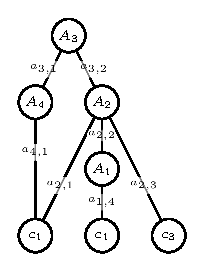
\includegraphics[width=0.25\textwidth]{images/decision_tree.eps}
	\caption{Example of a decision tree}
	\label{img:dec_tree}
\end{figure}

\begin{center}
	\begin{tabular}{>{\centering\arraybackslash}m{3in}>{\arraybackslash}m{3in}}
		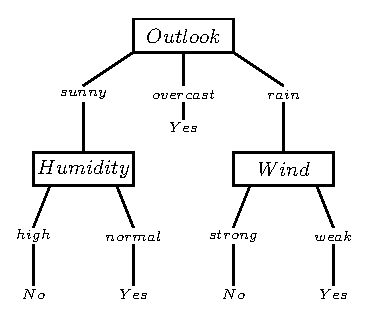
\includegraphics[width=0.3\textwidth ]{images/tennis_tree.eps} & Here's an example of a decision tree for the tennis problem. This representation is easy to classify a new instance that are not in the dataset, this tree defines rules such as: If the outlook is $overcast$, the output is $Yes$. The policy and the decisions are \textit{explicit}, and provides an explanation for the outcomes.
		\\
	\end{tabular}
\end{center}

In the hypothesis space $H$ we have all possible decision trees, that are finite for this kind of problems. Decision trees represent a disjunction of conjunctions of constraints, that can be easily described by looking at the tree, traveling the traces of the tree backward starting from the outcomes. An example is shown in figure \ref{img:conj_tree}. The recursive algorithm \ref{alg:dec_tree} works to compute one decision tree given the dataset $D$.\bigskip

\bigskip
\begin{figure}[h!]
	\centering
	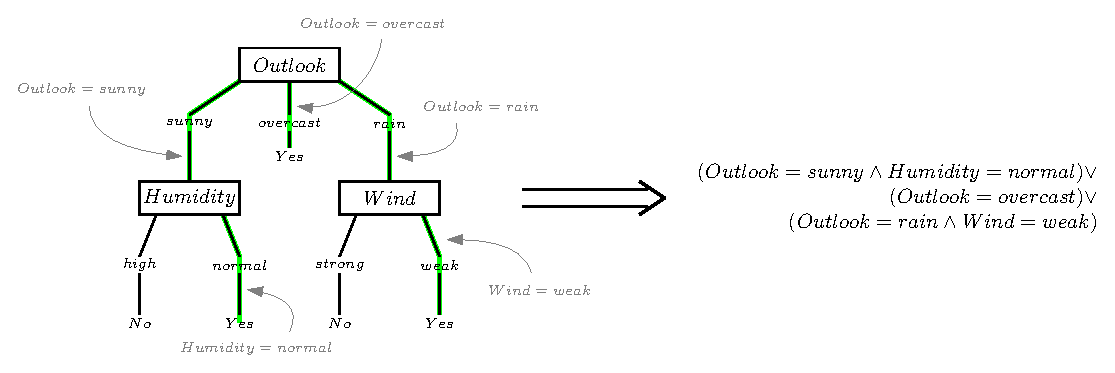
\includegraphics[width=1\textwidth]{images/conj_tree.eps}
	\caption{How paths in the tree transform into a logical formula}
	\label{img:conj_tree}
\end{figure}

\bigskip
\begin{algorithm}
	\caption{Computing Decision Tree for Binary Classification}\label{alg:dec_tree}
	\begin{algorithmic}
		\Require $D=\{(x_i,c_i)_i\}$, $Att=\{A_1\dots,A_m\}$
		\If{$\forall (x_i,c_i)\in D, \ \ c_i=+$}
		\State\Return $N(+)$
		\EndIf
		\If{$\forall (x_i,c_i)\in D, \ \ c_i=-$}
		\State\Return $N(-)$
		\EndIf
		\If{$Att=\emptyset$}
		\State $D_+=\{(x_i,c_i)\in D \ : \ c_i=+\}$
		\State $D_-=D\backslash D_+$
		\If{$|D_+|>|D_-|$}
		\State\Return  $N(+)$
		\EndIf
		\If{$|D_-|>|D_+|$}
		\State\Return  $N(-)$
		\EndIf
		\State\Return a random choice between $N(+)$ and $N(-)$
		\EndIf
		\State $A_i = \texttt{criteria}(Att)\in Att$
		\State we create a node $N(A_i)$
		\For{each $a_{i,j}\in A_i$}
		\State create an edge $N(A_i)\longrightarrow_{a_{i,j}} N(\ )$
		\State $D'=\{(x_i,c_i)\in D \ : \ x_i(A_i)=a_{i,j} \}$
		\State $N(\ )=$RecursiveCall($D',Att\backslash\{A_i\}$)
		\EndFor
		\State\Return the tree with root $N(A_i)$
	\end{algorithmic}
\end{algorithm}

We denote $N(+)$ a leaf node with the positive value, and $N(-)$ a leaf node with the negative value. If $A_i$ is an attribute, we denote $N(A_i)$ an intermediate node with the attribute $A_i$. We denote $N(\ )$ a node for which a value has not yet been assigned.

\bigskip
\section{The Information Gain}
The function \texttt{criteria}$(Att)$ choose one attribute from the remaining ones in the set $Att$, and defines decision policy. What is the best attribute to choose during the algorithm? That procedure defines the behavior of the algorithm. Let's consider the following example for a reduced version of the tennis problem, with the dataset shown in table \ref{tab:tennis_data}.

\begin{table}[h]
	\centering
	\caption{Dataset for the reduced tennis problem}
	\label{tab:tennis_data}
	\begin{tabular}{|c|c|c|c|}
		\hline
		{$Day$} & {$Outlook$} & {$Temperature$} & {$PlayTennis$} \\
		\hline
		D1      & Sunny       & Hot             & Yes            \\
		\hline
		D2      & Sunny       & Cold            & Yes            \\
		\hline
		D3      & Rain        & Hot             & No             \\
		\hline
		D4      & Rain        & Cold            & No             \\
		\hline
	\end{tabular}
\end{table}

If we apply the algorithm on this sample, there will be two possible solutions, one for the case where we choose $Outlook$ as the first choice for an attribute, one if we choose $Temperature$, the resulting trees as shown in figure \ref{img:tennis_criteria}.

\begin{figure}[h!]
	\centering
	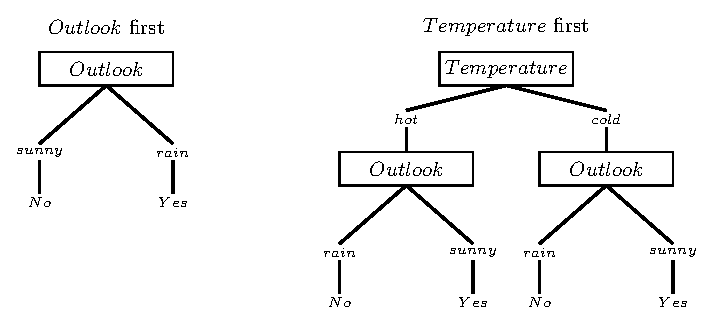
\includegraphics[width=0.7\textwidth]{images/tennis_criteria.eps}
	\caption{Different decision trees}
	\label{img:tennis_criteria}
\end{figure}

In general, not making the correct choice in the attributes can lead to a tree that incapsulate less information.  \begin{definition}
	Given an example dataset $S$, let $p_\oplus$ to be the proportion of positive examples in $S$, and $p_\ominus=1-p_\oplus$  the proportion of negative examples in $S$, the \textbf{entropy} of $S$ is the following value\begin{equation}
		Entropy(S)=-p_\oplus\log_2p_\oplus-p_\ominus\log_2p_\ominus.
	\end{equation}
\end{definition}
The curve of the $Entropy$ function is shown in figure \ref{fig:entropia_binaria}.
\begin{figure}[h!]
	\centering
	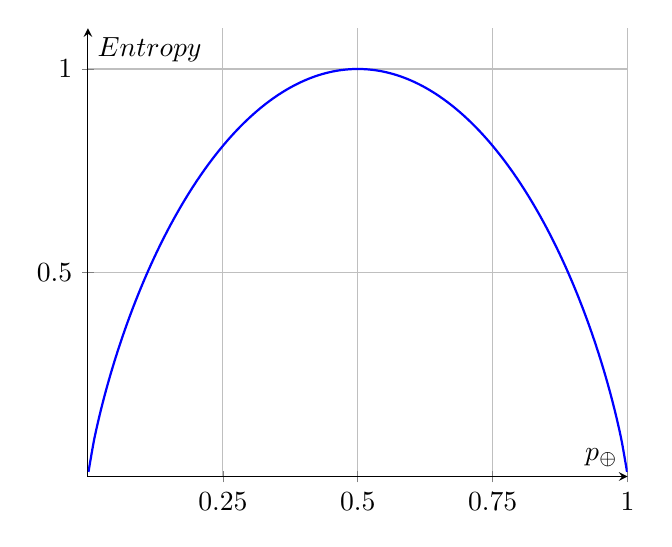
\begin{tikzpicture}
		\begin{axis}[
				% Impostazioni del grafico
				xlabel={$p_\oplus$},
				ylabel={$Entropy$},
				xmin=0, xmax=1, % Dominio della funzione
				ymin=0, ymax=1.1, % Imposta un intervallo comodo per l'asse Y
				grid=both, % Mostra la griglia
				axis lines=middle, % Assi centrati
				xtick={0, 0.25, 0.5, 0.75, 1},
				ytick={0, 0.5, 1},
				domain=0.001:0.999, % Evita x=0 e x=1, dove log è indefinito
				samples=100, % Numero di punti per una curva più liscia
			]
			\addplot[
				blue,
				thick,
				smooth
			]
			{
				-(x * (ln(x) / ln(2)))
				- ((1-x) * (ln(1-x) / ln(2)))
			};
		\end{axis}
	\end{tikzpicture}
	\caption{The curve of the $Entropy$ function}
	\label{fig:entropia_binaria}
\end{figure}

The entropy is minimum if we have all positive samples or all negative samples. The goal is to reduce the entropy of a dataset. We can partition the dataset in function of the different attributes, and then calculate the entropy for all the partitions. \bigskip

Given the table \ref{tab:tennis_data}, we can create two partitions, one by selecting $Outlook$, and one by selecting $Temperature$, as shown in figure \ref{img:partitions}.

\begin{figure}[h!]
	\centering
	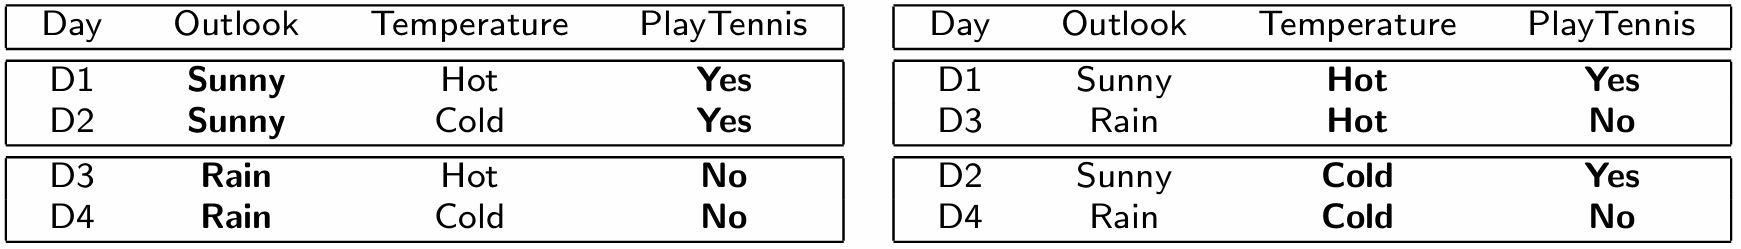
\includegraphics[width=0.9\textwidth]{images/partitions.png}
	\caption{Partitions of the dataset}
	\label{img:partitions}
\end{figure}

Splitting the dataset with outlook will generate two subsets with all positive/negative examples, so this two subsets will have an entropy of zero. In the other case, with temperature, the entropy will be 1.\bigskip

\noindent In the case of multi-valued target function (classification problem that is not binary), we can define the proportion of each class, denoted $p_i$, with $n$ classes, the entropy is\begin{equation}
	Entropy(S)=\sum_{i=1}^n-p_i\log_2p_i.
\end{equation}
\textbf{Note}: We define $0\log_20=0$.
\begin{definition}
	Given an example set $S$ and an attribute $A$, we define the \textbf{information gain} as the expected reduction in entropy of $S$ caused by knowing the value of the attribute $A$\begin{equation}
		Gain(S,A)=Entropy(S)-\sum_{v\in A}\frac{|S_v|}{|S|}Entropy(S_v)
	\end{equation}
	where\begin{equation}
		S_v=\{s\in S \ : \ s(A)=v\}
	\end{equation}
\end{definition}

If we take in example the dataset in the table \ref{tab:tennis_data_big}, we see that it have 9 positive samples and 5 negative samples, the entropy of the set is \begin{equation}
	-\frac{9}{14}\log_2\left(\frac{9}{14}\right)-\frac{5}{14}\log_2\left(\frac{5}{14}\right)=0.94
\end{equation}
We want to calculate the information gain for the attribute $Wind$, that can be $Weak$ or $Strong$. If we partition the sub-dataset for this attribute, we get one dataset with 6 positive values and 2 negative values, and a sub-dataset with 3 positive values and 3 negative values.

\bigskip
\begin{table}[h]
	\centering
	\caption{Split Dataset for the tennis problem}
	\label{tab:tennis_data_big_split}
	\begin{tabular}{cccccc}
		\toprule
		$Outlook$ & $Temperature$ & $Humidity$ & \textbf{Wind} & $PlayTennis$ \\
		\midrule
		Sunny     & Hot           & High       & Weak          & No           \\
		Overcast  & Hot           & High       & Weak          & Yes          \\
		Rain      & Mild          & High       & Weak          & Yes          \\
		Rain      & Cool          & Normal     & Weak          & Yes          \\
		Sunny     & Mild          & High       & Weak          & No           \\
		Sunny     & Cool          & Normal     & Weak          & Yes          \\
		Rain      & Mild          & Normal     & Weak          & Yes          \\
		Overcast  & Hot           & Normal     & Weak          & Yes          \\

		\bottomrule
	\end{tabular}
	\begin{tabular}{cccccc}
		\toprule
		$Outlook$ & $Temperature$ & $Humidity$ & \textbf{Wind} & $PlayTennis$ \\
		\midrule
		Sunny     & Hot           & High       & Strong        & No           \\
		Rain      & Cool          & Normal     & Strong        & No           \\
		Overcast  & Cool          & Normal     & Strong        & Yes          \\
		Sunny     & Mild          & Normal     & Strong        & Yes          \\
		Overcast  & Mild          & High       & Strong        & Yes          \\
		Rain      & Mild          & High       & Strong        & No           \\
		\bottomrule
	\end{tabular}
\end{table}

we have that\begin{align}
	 & |S_{weak}|=8            \\
	 & |S_{strong}|=6          \\
	 & |S|=14                  \\
	 & Entropy(S_{weak})=0.811 \\
	 & Entropy(S_{strong})=1
\end{align}
The information gain is\begin{align}
	 & Gain(S,Wind)=Entropy(S)-\frac{8}{14}Entropy(S_{weak})-\frac{6}{14}Entropy(S_{strong}) \\
	 & =0.94-\frac{8}{14}0.811-\frac{6}{14}=0.048.
\end{align}

This is a little information gain. A possible criteria for the choice of the next attribute in the algorithm \ref{alg:dec_tree}, is to select the attribute with the highest information gain, in the case of the dataset \ref{tab:tennis_data_big}, we have that\begin{align}
	 & Gain(S,Outlook)=0.245     \\
	 & Gain(S,Humidity)=0.151    \\
	 & Gain(S,Wind)=0.048        \\
	 & Gain(S,Temperature)=0.029
\end{align}

\bigskip
\noindent We call \texttt{ID3} the decision tree algorithm with the information gain criteria \ref{alg:ID3} . This algorithm can be seen as an algorithm that makes a search in the space of all possible hypothesis/decision trees.

\bigskip
\begin{algorithm}
	\caption{ID3 Decision Tree Learning}\label{alg:ID3}
	\begin{algorithmic}
		\Require Examples, Target\_attribute, Attributes
		\Ensure Decision Tree
		\State create a \textbf{Root} node for the tree
		\If{all Examples are positive}
		\State \Return node \textbf{Root} with label $+$
		\ElsIf{all Examples are negative}
		\State \Return node \textbf{Root} with label $-$
		\ElsIf{Attributes is empty}
		\State \Return node \textbf{Root} with label = most common value of \textit{Target\_attribute} in \textit{Examples}
		\Else
		\State $A \leftarrow$ best attribute for splitting \textit{Examples}
		\State assign $A$ as decision attribute for \textbf{Root}
		\For{each value $v_i$ of $A$}
		\State add a branch from \textbf{Root} corresponding to $A = v_i$
		\State $Examples_{v_i} \leftarrow$ subset of \textit{Examples} with $A = v_i$
		\If{$Examples_{v_i}$ is empty}
		\State add a leaf with label = most common value of \textit{Target\_attribute} in \textit{Examples}
		\Else
		\State add subtree $\text{ID3}(Examples_{v_i}, \ Target\_attribute, \ Attributes \setminus \{A\})$
		\EndIf
		\EndFor
		\EndIf
	\end{algorithmic}
\end{algorithm}

\bigskip
The hypothesis space of decision trees is \textit{complete}, and we can represent all possible subsets of the input space. The algorithm returns one single hypothesis that is consistent with the dataset, this algorithm cannot find the global optimum function but a local minima.
This algorithm is not incremental and uses all the training set at each step.

\newpage
\section{Issues in Decision Trees}
We have to consider the following problems:\begin{itemize}
	\item determining how deeply to grow the decision tree
	\item handling continuous attributes
	\item choosing appropriate attribute selection rule
	\item handling training data with missing attribute values
	\item handling attribute with different ''cost''.
\end{itemize}

\bigskip
\noindent Let $D$ to be the dataset shown in table \ref{tab:tennis_data_big}, we consider \begin{equation}
	D'=D\cup \left\langle  sunny,hot,normal,strong, PlayTennis=No\right\rangle
\end{equation}

\noindent\texttt{ID3} will generate two different decision trees $T,T'$ for the different dataset $D,D'$. The question is:\begin{quote}
	is $T'$ in general a better solution for this learning problem?
\end{quote}

In the general case, we have a dataset $D$ containing noisy data, and two decision trees $T$ and $T'$ obtained with different configurations of an \texttt{ID3}-like algorithm, where\begin{equation}
	accuracy_D(T')>accuracy_D(T)
\end{equation}
we don't know if $T'$ is a better solution, we should check the condition on a test set $S$\begin{equation}
	accuracy_S(T')>accuracy_S(T).
\end{equation}
Generally, the trend in figure \ref{img:trees_overfitting} is observed.\bigskip

\begin{figure}[h!]
	\centering
	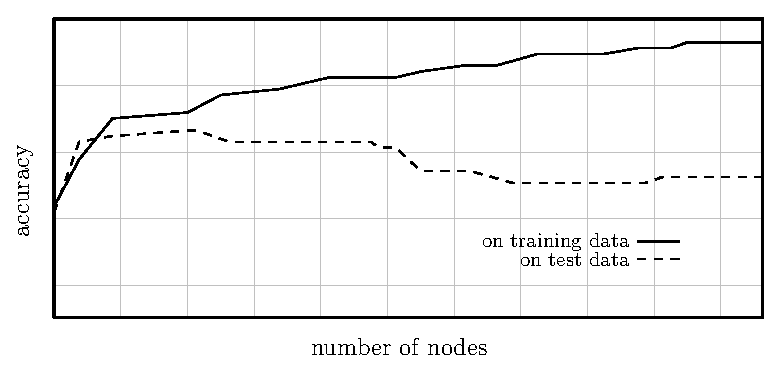
\includegraphics[width=0.7\textwidth]{images/trees_overfitting.eps}
	\caption{Decision trees overfitting}
	\label{img:trees_overfitting}
\end{figure}


To avoid overfitting, we should stop to grow the tree when the data split is not statistically significant, or could grow a full tree and then apply the \textit{post-prune}. With \textbf{pruning} we define the replacement of a sub-tree with a leaf node labelled as the most common class among samples filtered to the node.\bigskip

\begin{algorithm}
	\caption{Post Pruning}\label{alg:pruning}
	\begin{algorithmic}
		\Require a dataset $D$
		\State split data set in training $D_T$ and validation $D_V$
		\State generate a tree $T$ using the data set $D_T$
		\While{accuracy is not decreasing}
		\State  Evaluate the impact of pruning each node on the validation set
		\State Greedily remove the one that most improves validation on accuracy
		\EndWhile
	\end{algorithmic}
\end{algorithm}

If the dataset is limited, reducing the set of training examples (used
as validation examples) can give bad results.\bigskip

Decision trees can be expanded to \textit{continuous values}, for example, if temperature is expressed in degrees, we could introduce a variation of the tree that will generate some ''test'' in terms of intervals\begin{itemize}
	\item $Temperature=82.5$
	\item $(Temperature > 72.3) = True,False$
\end{itemize}
So this decision trees will have tests on equalities and tests on real values. There are also several other ways of defining the criteria for selecting the best attributes to include as a node, there are other measures than the information gain. We cannot say that one is always better, it depends on the problem.\bigskip

A dataset may have some samples with \textit{missing} attributes, for example:
\begin{center}
	\begin{tabular}{|c|c|c|c|}
		\hline
		{$Day$} & {$Outlook$} & {$Temperature$} & {$PlayTennis$} \\
		\hline
		D1      & Sunny       & UNKNOWN         & Yes            \\
		\hline
		D2      & Sunny       & UNKNOWN         & Yes            \\
		\hline
		D3      & UNKNOWN     & Hot             & No             \\
		\hline
		D4      & Rain        & Cold            & No             \\
		\hline
	\end{tabular}
\end{center}
in such case, with decision trees we can use the samples by adding some information to replace the missing values\begin{itemize}
	\item If a node $n$ tests an attribute $A$, we assign the most common value of $A$ among other examples sorted to node $n$.
	\item We can assign the most common value for $A$ among the other examples with the same target value.
\end{itemize}

\bigskip
There are other algorithms based on decision trees:\begin{itemize}
	\item we can generate a set of decision trees (called \textbf{forest}) with some random criteria and integrates their values into a final result.
	\item that integration of result could occur as a majority vote (most common class returned by all the trees)
	\item random forest are less sensitive to overfitting.
\end{itemize}

\chapter{Probabilistic Models}

\section{Probability Recap}

Consider the following action:
\begin{equation}
	A_t = \text{ leave the house $t$ minutes before the flight.}
\end{equation}

If we apply this action, what will be the answer to the question:
\begin{quote}
	Will the action $A_t$ get me to the airport on time?
\end{quote}

The answer cannot be a simple \textit{Yes} or \textit{No}, since it depends on several uncertain factors (traffic conditions, accidents, weather, etc.).

\smallskip
\textbf{Probability} provides a way to represent and reason about such uncertainty:
\begin{itemize}
	\item Given the available evidence, $A_{25}$ will get me to the airport on time with probability $0.04$;
	\item Given the available evidence, $A_{60}$ with probability $0.84$;
	\item Given the available evidence, $A_{1440}$ (leaving one day early) with probability $0.999$.
\end{itemize}

In this context, the set of all possible outcomes of an experiment is called the \textbf{sample space}, denoted by $\Omega$.
Each element $\omega \in \Omega$ represents one possible elementary event (a specific configuration of outcomes).

\begin{definition}
	A \textbf{Discrete Probability Space} is a tuple $(\Omega, \mathcal A, \Prob)$ where:
	\begin{itemize}
		\item $\Omega$ is the sample set of elementary events;
		\item $\mathcal A \subseteq \mathcal P(\Omega)$ is a \textbf{$\sigma$-algebra}, i.e. the collection of all events for which a probability can be defined.
		      It satisfies:
		      \begin{itemize}
			      \item $\Omega \in \mathcal A$
			      \item $A \in \mathcal A \implies A^C = \Omega \setminus A \in \mathcal A$
			      \item if $\{A_i\} \subset \mathcal A$ is countable, then $\bigcup_i A_i \in \mathcal A$.
		      \end{itemize}
		\item $\Prob$ is the \textbf{probability measure}, a function $\Prob: \mathcal A \rightarrow [0,1]$ that assigns a probability to each event and satisfies:
		      \begin{itemize}
			      \item $\Prob(\Omega) = \displaystyle\sum_{\omega \in \Omega} \Prob(\{\omega\}) = 1$
			      \item for any countable collection of disjoint events $\{A_i\}$:
			            \begin{equation}
				            \Prob\left(\bigcup_i A_i\right) = \sum_i \Prob(A_i).
			            \end{equation}
		      \end{itemize}
	\end{itemize}
\end{definition}

\bigskip
Intuitively, a probability space provides the formal structure for describing randomness:
$\Omega$ defines what can happen, $\mathcal A$ defines what we can measure, and $\Prob$ tells us how likely each event is.

\begin{definition}
	Given a probability space $(\Omega, \mathcal A, \Prob)$, a \textbf{random variable} is a function
	\[
		X : \Omega \rightarrow Y,
	\]
	that assigns a numerical or categorical value to each possible outcome $\omega \in \Omega$.
\end{definition}

\noindent
The probability measure $\Prob$ induces a \textbf{probability distribution} on the values of $X$:
\begin{equation}
	\Prob(X = x_i) = \sum_{\omega \in \Omega \, : \, X(\omega) = x_i} \Prob(\omega),
\end{equation}
that is, the probability that $X$ takes value $x_i$ is the sum of probabilities of all events leading to that outcome.

\bigskip
\begin{definition}
	Given a probability space $(\Omega, \mathcal A, \Prob)$, a \textbf{proposition} $a$ is an event in $\mathcal A$, associated with a random variable
	\[
		A : \Omega \rightarrow \{True, False\}
	\]
	such that
	\[
		a := A \text{ is True} := \{\omega \in \Omega \, : \, A(\omega) = True\}.
	\]
\end{definition}

\noindent
Propositions correspond to logical statements about the world (e.g., “the flight is on time”).
We can combine them using logical connectives:
\begin{align}
	 & \lnot a := A \text{ is False} := \{\omega \in \Omega : A(\omega) = False\}                                     \\
	 & a \land b := A \text{ and } B \text{ are True} := \{\omega : A(\omega)=B(\omega)=True\}                        \\
	 & \lnot a \lor b := A \text{ is False or } B \text{ is True} := \{\omega : A(\omega)=False \lor B(\omega)=True\}
\end{align}

Since each proposition is an event, we can compute its probability:
\begin{equation}
	\Prob(\lnot a \lor b) = \sum_{\omega \in \Omega : A(\omega)=False \lor B(\omega)=True} \Prob(\omega).
\end{equation}

\bigskip
Finally, recall that the probability distribution $\mathcal D$ defined in Definition~\ref{def:prob_distr} can also be interpreted as the distribution \emph{induced} by a random variable $X:\Omega \to Y$, assigning a probability to each possible value in $\mathcal P(Y)$.

We will give now an example of a probability space. Let's consider the rolling of a dice, in this case we have\begin{itemize}
	\item the sample set $\Omega=\{1,2,3,4,5,6\}$
	\item the $\sigma$-algebra $\mathcal A = \{\{1\},\{1,2\}\dots\}$
	\item the probability $\Prob$ defined as follows\begin{equation}
		      \forall\omega\in \Omega, \ \Prob(\{\omega\})=\frac{1}{6}.
	      \end{equation}
\end{itemize}

The probability of getting an odd number is
\begin{equation}
	\Prob(\{1,3,5\})=\Prob(\{1\})+\Prob(\{3\})+\Prob(\{5\})=\frac{1}{2}
\end{equation}

Let's consider the following random variable
\begin{align}
	 & X:\Omega\rightarrow\{-20,30\}    \\
	 & X(\omega)=30\iff\omega\in\{1,2\}
\end{align}

$X$ represents a gamble on the dice, if the result is less than 3, the player wins 30 euros, else, he loses 20 euros. The probability of winning is
\begin{equation}
	\Prob(\{1,2\})=\frac{1}{3}.
\end{equation}

If we have $n$ random variables $\{X_i\}$, it is possible to consider the \textbf{joint probability distribution}, inducted by the joint probability function.

Let $X_1,X_2$ to be two distinct random variables on two distinct probability spaces
\begin{align}
	 & X_1:\Omega_1\rightarrow Y_1 \text{ for the space }(\Omega_1,\mathcal A_1,\Prob_1) \\
	 & X_2:\Omega_2\rightarrow Y_2 \text{ for the space }(\Omega_2,\mathcal A_2,\Prob_2)
\end{align}
where $\mathcal D_1$ is the distribution on $X_1$ and $\mathcal D_2$ is the distribution on $X_2$, the joint distribution $\mathcal D$ is defined as follows:
\begin{align}
	 & \text{let }x_1\in Y_1, \ \ x_2\in Y_2                                                                                                 \\
	 & \mathcal D(X_1=x_1, \ X_2=x_2)=\Prob(\{(\omega_1,\omega_2)\in\Omega_1\times\Omega_2 \ : \ X_1(\omega_1)=x_1\land X_2(\omega_2)=x_2\})
\end{align}
where $\Prob:\mathcal A_1\times\mathcal A_2\rightarrow[0,1]$ is the joint probability and defines the probability that two events from the different probability space occurs.

\bigskip
If $a$ and $b$ are two events/propositions, we define the \textbf{conditional probability} as follows:
\begin{equation}
	\Prob(a|b)=\frac{\Prob(a\land b)}{\Prob(b)}, \ \ \text{if }\Prob(b)\ne0
\end{equation}
it represents the probability that $a$ occurs knowing that $b$ is true.

The \textbf{product rule} holds:
\begin{equation}
	\Prob(a,b)=\Prob(a\land b)=\Prob(a|b)\Prob(b)=\Prob(b|a)\Prob(a)
\end{equation}

The following equality is called \textbf{chain rule} and is needed to calculate the probability that multiple events $A_1,A_2\dots A_n$ occurs:
\begin{align}
	 & \Prob(A_1,A_2\dots A_n)=\prod_{i=1}^n\Prob(A_i|A_1,\dots A_{i-1})=
	\\ &\prod_{i=1}^n\left( A_i|\bigcap_{j=1}^{i-1} A_j \right).
\end{align}

\textbf{Note}: We will use the following abuse of notation, if $\Prob$ is the probability function for a probability space $(\Omega,\mathcal A,\Prob)$, and $X$ is a random variable on $\Omega$, we use the same symbol $\Prob$ to denote a probability distribution on $X$
\begin{align}
	 & \Prob(A), \ A\in\mathcal A \ \ \text{in this context $\Prob$ is the probability function} \\
	 & \Prob(X=x_i) \ \ \text{in this context $\Prob$ is the probability distribution.}
\end{align}

\begin{theorem}
	Let's consider a probability space $(\Omega,\mathcal A, \Prob)$, let $A\in \Omega$ and let $\{B_1,B_2\dots B_n\}$ to be a partition of $\Omega$.
	The \textbf{Total Probability} formula states that:
	\begin{equation}
		\Prob(A)=\sum_{i=1}^n\Prob(A\cap B_i)
	\end{equation}
	since $\Prob(A\cap B_i)=\Prob(A|B_i)\Prob(B_i)$ we have
	\begin{equation}
		\Prob(A)=\sum_{i=1}^n\Prob(A|B_i)\Prob(B_i)
	\end{equation}
\end{theorem}

Let $X=\{X_1,X_2\dots X_n\}$ a finite set of random variables, and let $\omega$ be an assignment of all the variables
\begin{align}
	 & \omega=(x_1,x_2\dots x_n)                     \\
	 & \omega\in\Omega=X_1\times X_2\dots \times X_n \\
	 & x_1\in X_1                                    \\
	 & x_2\in X_2                                    \\
	 & \vdots                                        \\
	 & x_n\in X_n.
\end{align}

There exists a joint probability distribution $\Prob$ on $\Omega$. Let $\phi$ to be a proposition defined in terms of $X_1\dots X_n$, for example
\begin{equation}
	\phi=x_1\lor x_2 \land \lnot x_3
\end{equation}
$\phi$ is satisfied by all the events $\Omega_\phi$:
\begin{equation}
	\Omega_\phi=\{\omega\in \Omega \ : \ \omega \text{ makes } \phi \text{ true }\}
\end{equation}
the \textbf{Inference by Enumeration} formula states that, the probability that $\phi$ is satisfied is
\begin{equation}
	\Prob(\phi)=\sum_{\omega\in  \Omega_\phi}\Prob(\omega)
\end{equation}

\begin{definition}
	Given a probability space $(\Omega,\mathcal A,\Prob)$, and two events $A,B\in\mathcal A$, we say that $A$ and $B$ are \textbf{independent} if and only if
	\begin{equation}
		\Prob(A, B)=\Prob(A\land B)=\Prob(A)\Prob(B).
	\end{equation}
\end{definition}

\subsection{Conditional Probability and Bayes' Theorem}

In many real-world problems, we are not interested in the probability of an event occurring in isolation, but rather in the probability of one event \emph{given} that another has occurred.
This leads to the concept of \textbf{conditional probability}.

\begin{definition}
	Given two events $A,B \in \mathcal A$ with $\Prob(B) > 0$, the \textbf{conditional probability} of $A$ given $B$ is defined as:
	\begin{equation}
		\Prob(A|B) = \frac{\Prob(A \cap B)}{\Prob(B)}.
	\end{equation}
\end{definition}

This definition allows us to update our belief about $A$ once we know that $B$ has occurred.

\bigskip
\begin{theorem}
	Given a probability space $(\Omega,\mathcal A,\Prob)$ and two events $A,B\in\mathcal A$, the \textbf{Bayes' Theorem} states that:
	\begin{equation}
		\Prob(A|B) = \frac{\Prob(B|A)\Prob(A)}{\Prob(B)}.
	\end{equation}
\end{theorem}

Bayes’ theorem provides a way to \textit{invert} conditional probabilities — i.e., to compute $\Prob(A|B)$ in terms of $\Prob(B|A)$.
This is fundamental in machine learning, where we often want to infer the probability of a \emph{hidden cause} (e.g., a class label or model parameter) given an \emph{observed effect} (e.g., data).

\bigskip
\textbf{Example intuition.}
If $A$ represents “the email is spam” and $B$ represents “the email contains the word ‘discount’,” then $\Prob(B|A)$ is easy to estimate (how often spam emails mention “discount”),
while $\Prob(A|B)$ — the probability that an email is spam given that it contains “discount” — can be inferred using Bayes’ theorem.

\bigskip
\subsection{Likelihood and the Maximum Likelihood Principle}

In machine learning and statistics, we often deal with random variables $X$ and $Y$, where $X$ represents the unknown parameter or cause, and $Y$ represents the observed data.
Given an observation $Y = y_i$, we want to determine which value of $X$ is most likely responsible for it.

\bigskip
The \textbf{likelihood function} of $X$ given an observation $y_i$ is defined as:
\begin{equation}
	\mathcal{L}(x) = \Prob(Y = y_i | X = x),
\end{equation}
which represents how “compatible” each value of $x$ is with the observed data $y_i$.

\bigskip
The \textbf{maximum likelihood estimate (MLE)} seeks the value of $x$ that maximizes this likelihood:
\begin{equation}
	\hat{x}_{ML} = \arg\max_x \Prob(X = x | Y = y_i) = \arg\max_x \frac{\Prob(Y = y_i | X = x)\Prob(X = x)}{\Prob(Y = y_i)}.
\end{equation}

If all possible values of $X$ are assumed to be equally likely (uniform prior), then $\Prob(X=x)$ is constant and can be ignored.
Since $\Prob(Y=y_i)$ is also constant with respect to $x$, we obtain:
\begin{equation}
	\hat{x}_{ML} = \arg\max_x \Prob(Y = y_i | X = x).
\end{equation}

\noindent
This is the essence of the \textbf{Maximum Likelihood Principle}:
\begin{quote}
	Choose the parameters or hypotheses that make the observed data most probable.
\end{quote}

\section{Bayesian Learning}

The Bayesian approach introduces a probabilistic framework for learning, in which uncertainty about hypotheses and predictions is represented explicitly through probabilities.
Instead of committing to a single “best” model derived only from data, Bayesian learning updates our belief about all possible hypotheses as new evidence is observed, represented in a distribution.

\bigskip
\noindent
Consider a classification problem defined by a target function:
\begin{equation}
	f : X \rightarrow V,
\end{equation}
where $V$ is a finite set of possible classes.
For each instance $x \in X$, and a given dataset $D$, we are interested in the probability
\begin{equation}
	\Prob(v | x, D), \qquad v \in V,
\end{equation}
that the correct label of $x$ is $v$ given the evidence provided by $D$.
The learned function can therefore be defined as:
\begin{equation}
	\hat f(x) = \arg\max_{v \in V} \Prob(v | x, D) = v^*,
\end{equation}
that is, we predict the class with the highest posterior probability.
In general, it may be useful to compute the entire distribution $\Prob(v | x, D)$ for all $v \in V$, as it reflects our confidence in each possible classification.

\bigskip
\subsection{Posterior Probability over Hypotheses}

To model how data affect our confidence in each hypothesis, we define:
\begin{equation}
	\Prob(h | D),
\end{equation}
the probability that a hypothesis $h \in H$ is correct given the observed dataset $D$.
Applying Bayes’ theorem:
\begin{equation}
	\Prob(h | D) = \frac{\Prob(D | h)\Prob(h)}{\Prob(D)}.
\end{equation}

\begin{itemize}
	\item $\Prob(h)$ — the \textbf{prior probability}: our belief in $h$ before observing any data.
	\item $\Prob(D | h)$ — the \textbf{likelihood}: how probable the data $D$ are if hypothesis $h$ were true.
	\item $\Prob(D)$ — the \textbf{evidence}: a normalizing constant ensuring probabilities sum to $1$.
	\item $\Prob(h | D)$ — the \textbf{posterior probability}: our updated belief in $h$ after observing $D$.
\end{itemize}

\noindent
Bayesian learning can therefore be summarized as:
\[
	\text{posterior} \propto \text{likelihood} \times \text{prior}.
\]
This principle expresses how learning combines prior knowledge with new observations.

\bigskip
\subsection{The Maximum a Posteriori (MAP) Hypothesis}

In practice, it is often infeasible to compute or store the entire posterior distribution over $H$.
A common approach is to select the most probable hypothesis according to the posterior:
\begin{equation}
	h_{MAP} = \arg\max_{h \in H} \Prob(h | D)
	= \arg\max_{h \in H} \frac{\Prob(D | h)\Prob(h)}{\Prob(D)}
	= \arg\max_{h \in H} \Prob(D | h)\Prob(h).
\end{equation}

\noindent
The denominator $\Prob(D)$ can be dropped, as it is constant with respect to $h$.
The resulting \textbf{Maximum a Posteriori} (MAP) estimate therefore finds the hypothesis that both fits the observed data and aligns with our prior expectations.

\bigskip
If all hypotheses are equally likely a priori (i.e., the prior $\Prob(h)$ is uniform), the MAP estimate reduces to the maximum likelihood solution.
Thus, Bayesian learning generalizes maximum likelihood estimation by incorporating prior knowledge and explicitly reasoning about uncertainty.

\bigskip
This probabilistic viewpoint not only provides a principled way to handle noisy or incomplete data, but also forms the theoretical basis for models such as Naive Bayes classifiers, Bayesian networks, and Gaussian processes.

\subsection{Bayes Optimal Classifier}

The hypothesis $h_{MAP}$ represents the single most probable hypothesis given the data $D$.
However, this does not necessarily guarantee that the corresponding prediction is the best one.
In fact, $h_{MAP}$ ignores the uncertainty associated with the other hypotheses in $H$.

To obtain the truly optimal classifier — in the Bayesian sense — we consider the expected prediction over all possible hypotheses, weighted by their posterior probabilities.

\bigskip
\noindent
For each class $v_j \in V$, the probability that the correct label of $x$ is $v_j$ given the dataset $D$ can be expressed using the law of total probability:
\begin{equation}
	\Prob(v_j|x,D) = \sum_{h_i \in H} \Prob(v_j|x,h_i,D) \Prob(h_i|x,D).
\end{equation}
Since the data $D$ are already known, the first term does not depend on $D$ once $h_i$ is fixed, and the second term does not depend on $x$:
\[
	\Prob(v_j|x,h_i,D) = \Prob(v_j|x,h_i), \quad \Prob(h_i|x,D) = \Prob(h_i|D).
\]
Hence,
\begin{equation}
	\Prob(v_j|x,D) = \sum_{h_i \in H} \Prob(v_j|x,h_i)\Prob(h_i|D).
\end{equation}

\bigskip
\noindent
The \textbf{Bayes Optimal Classifier} is then defined as:
\begin{equation}
	v_{OB}(x) = \arg\max_{v_j \in V} \sum_{h_i \in H} \Prob(v_j|x,h_i)\Prob(h_i|D).
\end{equation}
\newpage
This classifier computes the posterior probability of each class by averaging over all hypotheses, weighted by how probable each hypothesis is after observing the data.
It is provably the best possible classifier under the same hypothesis space and available data — no other learner can achieve a lower expected error.

\bigskip
\noindent
\textbf{Example.}
Suppose we have three hypotheses $h_1, h_2, h_3$ with posterior probabilities:
\[
	\Prob(h_1|D)=0.4, \quad \Prob(h_2|D)=0.3, \quad \Prob(h_3|D)=0.3,
\]
and the class probabilities predicted by each hypothesis are:
\begin{align*}
	\Prob(\oplus|x,h_1) & =1, & \Prob(\ominus|x,h_1) & =0, \\
	\Prob(\oplus|x,h_2) & =0, & \Prob(\ominus|x,h_2) & =1, \\
	\Prob(\oplus|x,h_3) & =0, & \Prob(\ominus|x,h_3) & =1.
\end{align*}
The posterior class probabilities are:
\begin{align*}
	\Prob(\oplus|x,D)  & = \sum_{i=1}^3 \Prob(\oplus|x,h_i)\Prob(h_i|D) = 0.4,  \\
	\Prob(\ominus|x,D) & = \sum_{i=1}^3 \Prob(\ominus|x,h_i)\Prob(h_i|D) = 0.6,
\end{align*}
so the Bayes optimal prediction is $v_{OB}(x) = \ominus$.
This shows that even though $h_{MAP}=h_1$, the optimal classifier considers the contribution of all hypotheses.

\bigskip
\noindent
In general, computing $v_{OB}(x)$ is infeasible because it requires iterating over the entire hypothesis space $H$, which may be extremely large or continuous.
For this reason, practical algorithms use approximations such as $h_{MAP}$ or the Naive Bayes model introduced later.

\bigskip
\subsubsection{The Candy Example}

To illustrate Bayesian updating, consider a simple generative model.
There are five bags of candies, each corresponding to a hypothesis $h_i$:
\begin{center}
	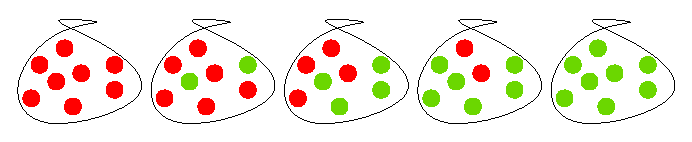
\includegraphics[width=0.7\textwidth]{images/candies.eps}
\end{center}

\noindent
Each $h_i$ specifies a different proportion of cherry ($c$) and lime ($l$) candies:
\begin{center}
	\begin{tabular}{c|c|c}
		$h_i$ & Description                & $\Prob(h_i)$ \\ \hline
		$h_1$ & $100\%$ cherry             & $0.10$       \\
		$h_2$ & $75\%$ cherry, $25\%$ lime & $0.20$       \\
		$h_3$ & $50\%$ cherry, $50\%$ lime & $0.40$       \\
		$h_4$ & $25\%$ cherry, $75\%$ lime & $0.20$       \\
		$h_5$ & $100\%$ lime               & $0.10$
	\end{tabular}
\end{center}

\noindent
Before observing any data, the probability of drawing a lime candy is:
\[
	\Prob(l) = \sum_{i=1}^{5}\Prob(l|h_i)\Prob(h_i) = 0.5.
\]

\noindent
Now suppose the first observed candy is lime, $D_1=\{l\}$.
Applying Bayes’ rule:
\[
	\Prob(h_i|D_1) = \frac{\Prob(D_1|h_i)\Prob(h_i)}{\Prob(D_1)} = \alpha \, \Prob(l|h_i)\Prob(h_i),
\]
\newpage
where $\alpha$ is a normalizing constant ensuring $\sum_i \Prob(h_i|D_1)=1$.
After updating for successive lime observations ($D_2=\{l,l\}$, $D_3=\{l,l,l\}$), the posterior shifts increasingly toward hypotheses with higher lime proportions.
Figure~\ref{img:candy_graph} shows this evolution.

\begin{figure}[h!]
	\centering
	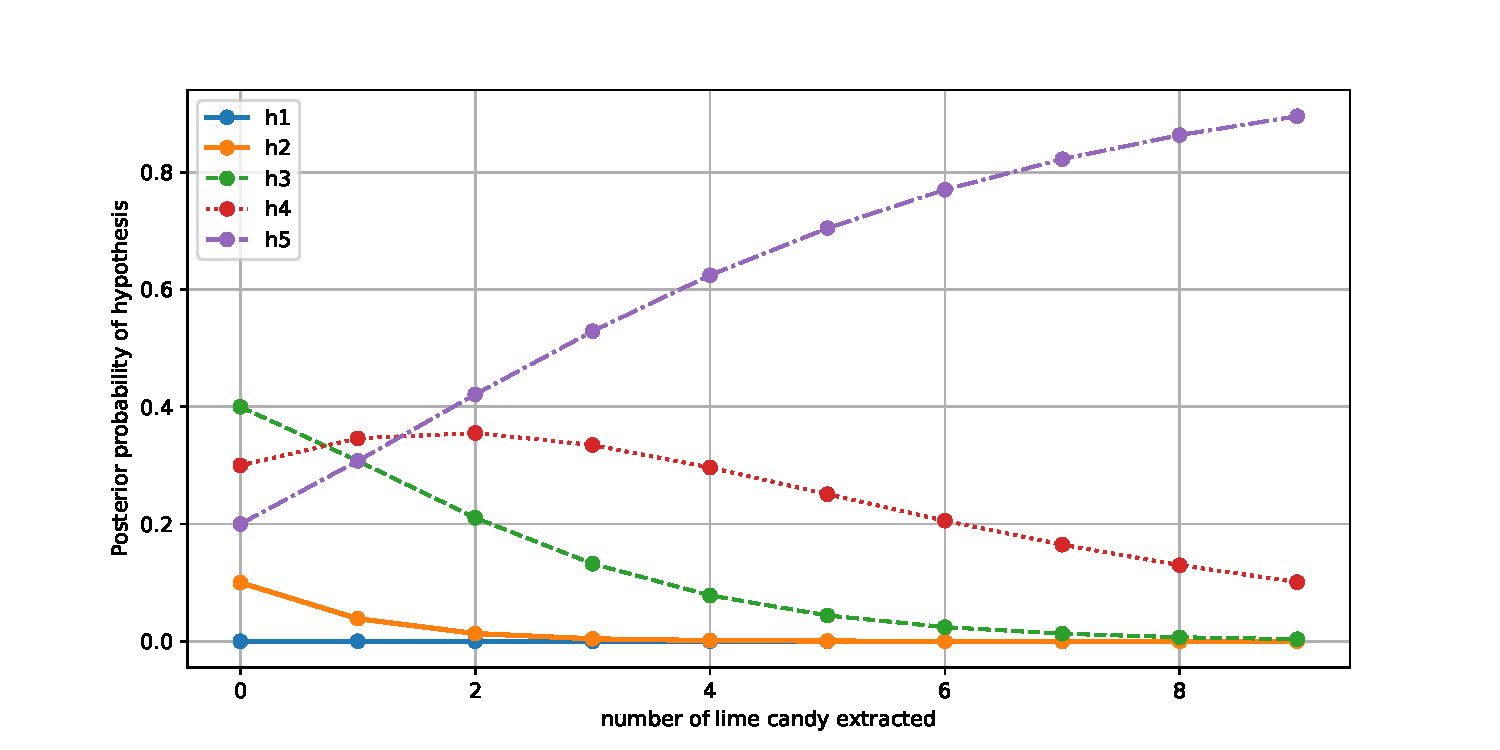
\includegraphics[width=0.8\textwidth]{images/candy_graph.pdf}
	\caption{Posterior probabilities for each hypothesis as lime candies are observed.}
	\label{img:candy_graph}
\end{figure}

\bigskip
\noindent
After three lime candies, the posterior probability that the next candy is lime is:
\[
	\Prob(l|D_3) = \sum_{i=1}^5 \Prob(l|h_i)\Prob(h_i|D_3) = 0.8.
\]
Notice that the $h_{MAP}$ hypothesis would be $h_5$ (100\% lime), yielding $\Prob(l|h_5)=1$, which overestimates the true probability — highlighting why averaging across hypotheses is more accurate.

\bigskip
\subsubsection{Continuous Hypothesis Space}

Now consider a continuous family of hypotheses $h_\theta$, where $\theta \in [0,1]$ represents the proportion of cherry candies:
\[
	\Prob(c|h_\theta)=\theta, \qquad \Prob(l|h_\theta)=1-\theta.
\]
Given a dataset $D$ with $c$ cherries and $l$ limes, the likelihood is:
\[
	\Prob(D|h_\theta)=\theta^c(1-\theta)^l.
\]
The log-likelihood is:
\[
	L(D,h_\theta)=c\log\theta + l\log(1-\theta),
\]
and maximizing it with respect to $\theta$ gives:
\[
	\theta^* = \frac{c}{c+l} = \frac{c}{|D|}.
\]
Thus, $h_{\theta^*}$ is the maximum likelihood hypothesis.
In more complex distributions, this maximization cannot always be performed analytically.

\bigskip
\subsection{Naive Bayes Classifier}

The Bayes Optimal Classifier provides the best possible predictions but is computationally impractical for large or continuous hypothesis spaces.
The Naive Bayes Classifier provides a simple yet powerful approximation by assuming that the input features are conditionally independent given the class.

\begin{definition}
	Two random variables $X$ and $Y$ are \textbf{conditionally independent} given $Z$ if:
	\begin{equation}
		\Prob(X,Y|Z) = \Prob(X|Z)\Prob(Y|Z).
	\end{equation}
\end{definition}

\noindent
Although this assumption is rarely true in real-world data, it leads to an efficient classifier that performs remarkably well in practice.

\bigskip
\noindent
Given a target function $f: X \rightarrow V$, where each instance $x \in X$ is described by attributes $x=(a_1,a_2,\dots,a_n)$, we wish to predict:
\[
	v_{NB}(x) = \arg\max_{v\in V}\Prob(v|a_1,a_2,\dots,a_n,D).
\]
By Bayes’ theorem:
\[
	\Prob(v|a_1,\dots,a_n,D) \propto \Prob(a_1,\dots,a_n|v,D)\Prob(v|D),
\]
and assuming conditional independence among the attributes:
\[
	\Prob(a_1,\dots,a_n|v,D) = \prod_{i=1}^n \Prob(a_i|v,D).
\]
Thus, the \textbf{Naive Bayes Classifier} becomes:
\[
	v_{NB}(x) = \arg\max_{v\in V}\Prob(v|D)\prod_{i=1}^n\Prob(a_i|v,D).
\]

\bigskip
\noindent
The probabilities are estimated from the dataset as:
\[
	\hat\Prob(v_j|D)=\frac{|D_{v_j}|}{|D|}, \qquad
	\hat\Prob(a_i^k|v_j,D)=\frac{|D_{a_i^k}|+mp}{|D_{v_j}|+m},
\]
where $p$ and $m$ represent prior knowledge and its confidence weight.

\bigskip
\noindent
Despite its simplicity and the unrealistic independence assumption, the Naive Bayes classifier performs surprisingly well in many domains.
Its success stems from the fact that even if individual probabilities are inaccurate, their relative magnitudes (which determine the $\arg\max$) often remain correct.

\subsection{Text Classification}
In this section we explain how to model a simple document classifier using the naive Bayes approach, the target function, given a document, returns the the class of that document (e.g. Scientific Article, Recipe, Poem, ecc...). This classifier have multiple application, in example:\begin{itemize}
	\item Spam classification for e-mail
	\item Sentiment analysis
\end{itemize}
Let $f$ to be the target function, $C=\{c_1,\dots c_k\}$ the set of the classes, and $Docs$ the set of documents. $D=\bigcup_{i=1}^n\{(doc_i,c_i)\}$ is the dataset. We want to compute\begin{equation}
	c_{NB}(doc)=\arg\max_{c_j\in C}\Prob(c_j|D)\Prob(doc|c_j,D).
\end{equation}
We want to express each document $doc$ as a ordered list of words, we define a vocabulary\begin{equation}
	V=\{w_1,w_2\dots w_n\}
\end{equation}
that contains all possible words $w_i$ that can appear in any document. Any document $doc_i\in Docs$ have a length (number of words) denoted $m_i$\begin{equation}
	doc_i=w_1w_2\dots w_{m_i}
\end{equation}
The probability that a document $doc_i$ is in class $c_j\in C$ given $D$ is\begin{equation}
	\Prob(doc_i|c_j,D)=\prod_{k=1}^{m_i}\Prob(p_k=w_k|c_j,D)
\end{equation}
where $\Prob(p_k=w_k|c_j|D)$ is the probability that, in a document $doc_i$ of class $c_j$, the word $p_k$ at position $k$ is $w_k$. We assume that the order of the words does not affect the probability\begin{equation}
	\forall,k,k' \ \ \ \Prob(p_k=w_k|c_j,D)=\Prob(p_{k'}=w_{k'}|c_j,D)
\end{equation}
so we consider only \begin{equation}
	\Prob(w_k|c_j,D)=\text{ probability that $w_k$ occurs in a document of class $c_j$ given $D$}.
\end{equation}
Each document can be represented as a $n$-dimensional vector, where the coordinate $i$ is equal to $k$ if in the document there are $k$ words $w_i\in V$. This representation looses the information about the order of the words. In this context, we denote a vector \begin{align}
	 & \mathbf d = (d_1,d_2\dots d_n) \\ &d_i = \text{ number of times words $w_i$ appear in $\mathbf d$}
\end{align}
we recall that $n=|V|$ is the number of distinct words in the vocabulary, the probability of classifying $\mathbf d$ as $c_j\in C$ given $D$ is\begin{equation}
	\Prob(\mathbf d|c_j,D)=\frac{n!}{d_1!\dots d_n!}\prod_{i=1}^{n}\Prob(w_i|c_j,D)^{d_i}
\end{equation}
we recall that $\Prob(w_i|c_j,D)$ is the probability of observing the word $w_i$ given that the document $\mathbf d$ belongs to the class $c_j$.  This probability is estimated with the maximum likelihood value:\begin{equation}
	\hat\Prob(\mathbf d|c_j,D)=\frac{\displaystyle
		\sum_{\mathbf d \in D}tf_{i,j}+\alpha
	}{\displaystyle
		\sum_{\mathbf d \in D}tf_{j}+\alpha n
	}
\end{equation}
where\begin{itemize}
	\item $tf_{i,j}$ is the all-term frequency that $w_i$ occurs in the document $\mathbf d$ given that $\mathbf d$ is of class $c_j$ within the document dataset $D$.
	\item $tf_{j}$ is the total number of words in all document of $D$ that belongs to the class $c_j$.
	\item $\alpha$ is a smoothing parameter.
\end{itemize}
The algorithm \ref{alg:text_classifier} describes the methods that estimate the probabilities to classify new documents.\bigskip

\begin{algorithm}
	\caption{Text Classifier}\label{alg:text_classifier}
	\begin{algorithmic}
		\Require a dataset of documents $D$, a set of classes $C$
		\State $V\longleftarrow$ all distinct words in $D$
		\For{each $c_j\in C$}
		\State $docs_j\longleftarrow$ subset of $D$ of document of class $c_j$
		\State $t_j\longleftarrow |docs_j|$
		\State $\hat\Prob(c_j)\longleftarrow \frac{t_j}{|D|}$
		\State $TF_j\longleftarrow$ total number of words in $docs_j$ (counting duplicates)
		\For{$w_i\in V$}
		\State $TF_{i,j}\longleftarrow$ total number of times that $w_i$ occurs in $docs_j$
		\State $\hat\Prob(w_i|c_j)\longleftarrow \frac{TF_{i,j}+1}{TF_j+|V|}$
		\EndFor
		\EndFor
	\end{algorithmic}
\end{algorithm}

After we got the probabilities $\hat\Prob$, we classify a new document $doc=w_1\dots w_{m}$ as follows\begin{equation}
	v_{NB}(doc)=\arg\max_{c_j\in C}\hat\Prob(c_j)\prod_{i=1}^{m}\hat\Prob(w_i|c_j)
\end{equation}

\section{Probabilistic Generative Models}
In Probabilistic Generative Models, the search of a solution is the determination of the best parameters $\btheta$ that define how samples are generated.
Rather than modeling every possible distribution, we restrict the hypothesis space to functions
\[
	\Prob(\mathbf x|c_k) = \Prob(\mathbf x|\btheta_k),
\]
where $\btheta_k$ contains the parameters of the distribution (such as means, variances or covariances).
\newline
Learning then consists of estimating these parameters from data, which determines the shape and flexibility of the model.
A higher number of parameters usually increases expressiveness but also the risk of overfitting and to be computationally expensive.

\bigskip
\subsection{Parametrized Hypothesis Space}
Given a target function
$$ f:X\rightarrow C $$
we have a \textbf{parametrized} hypothesis space if, the set of all possible solutions $H$, contains functions of the type
\begin{equation}
	y(x,\btheta)
\end{equation}
where $x\in X$ and $\btheta$ is the parameters of the function, an example is\begin{equation}
	y(x,\mathbf w)=y(x,(w_1,w_2,w_3,w_4))=\sum_{i=1}^4x^iw_i
\end{equation}

\bigskip
A model could also be \textbf{hyperparametrized}, if the set of possible solution is parameterized by some fixed values that can't change during the training. An example of hyper parameter could be the grade of the polynomials functions in the hypothesis space $H$.
\begin{align*}
	 & H=\left\{\sum_{i=1}^nw_ix^i\right\}     \\
	 & n\text{ is an hyperparameter}           \\
	 & w_1,\dots w_n\text{ are the parameters}
\end{align*}
Let's consider a classification problem, the function to learn is\begin{equation}
	f:X\rightarrow\{c_1,c_2\dots c_K\}
\end{equation}
where the input space is continuous: $X\subseteq\R^d$. We need to evaluate the probability that a given point is in a given class\begin{equation}
	\Prob(c_k|c,D) \ \ \ x\notin D
\end{equation}
since the dataset is fixed in this context, we can write directly \begin{equation}
	\Prob(c_k|c) \ \ \ x\notin D
\end{equation}
is implicit that the probability depends on the dataset. The \textit{main assumption} of this section is that there is a \textbf{Gaussian Distribution} over $x$, for each class $c_k$
\begin{equation}
	\Prob(x|c_k)=\mathcal N(x,\mu_k,\Sigma_k)
\end{equation}
where $\mu_k$ is the mean vector and $\Sigma_k$ is the covariance matrix. To emphasize and reiterate that certain quantities are vectors, bold letters will be used in the notation.
\begin{equation}
	\Prob(\mathbf x|c_k)=\mathcal N(\mathbf  x,\bmu_k,\Sigma_k)
\end{equation}

\paragraph{Why Gaussian Distributions?}
The assumption that each class follows a Gaussian distribution is mainly motivated by mathematical convenience and empirical effectiveness.
Gaussian densities can be estimated efficiently, they provide smooth continuous models, and under mild assumptions on the data (from the Central Limit Theorem) they offer a reasonable approximation for many real-world distributions.
Moreover, they lead to analytically tractable posterior probabilities and simple decision boundaries.

\subsection{Models for 2 Classes}
Let's consider the case with two classes
$$
	f:X\rightarrow\{c_1,c_2\}
$$
In this case, assuming that the distributions are gaussian, we have that
\begin{align}
	 & \Prob(\mathbf x|c_1)=\mathcal N(\mathbf x,\bmu_1,\Sigma_1) \\
	 & \Prob(\mathbf x|c_2)=\mathcal N(\mathbf x,\bmu_2,\Sigma_2)
\end{align}
we recall that
\begin{align}
	 & X\subset \R^d              \\
	 & \bmu_i,\mathbf x\in\R^d    \\
	 & \Sigma_i\in Mat(d\times d)
\end{align}
we also have
\begin{equation}
	\Prob(c_1)=p,  \ \ \ \ \Prob(c_2)=1-p
\end{equation}
now, we have to estimate the parameters $\bmu_1,\Sigma_2,\bmu_1,\Sigma_2,p$ to use $\Prob(\mathbf x|c_i)$ and make predictions on samples that are not in the dataset, since for the Bayes theorem:
\begin{align}
	 & \Prob(c_1|\mathbf x)=\frac{\Prob(\mathbf x|c_1)\Prob(c_1)}{\Prob(\mathbf x)} \\
	 & \Prob(c_2|\mathbf x)=\frac{\Prob(\mathbf x|c_2)\Prob(c_2)}{\Prob(\mathbf x)}
\end{align}
...
we get
\begin{align}
	 & \Prob(c_i|\mathbf x)=\frac{\Prob(\mathbf x|c_i)\Prob(c_i)}{\Prob(\mathbf x|c_1)\Prob(c_1)+\Prob(\mathbf x|c_2)\Prob(c_2)}= \\
	 & \frac{1}{1+\exp(-a(\mathbf x))}=\sigma(a(\mathbf x))
\end{align}
The $\sigma$ is called \textbf{sigmoid function}, which ''squeezes'' the values from $\R$ to $[0,1]$. By the assumption about the distribution, we now that
\begin{equation}
	a(\mathbf x)=\ln\left(\frac{\Prob(\mathbf x|c_1)\Prob(c_1)}{\Prob(\mathbf x|c_2)\Prob(c_2)}\right)=
	\ln\left(\frac{\mathcal N(\mathbf x,\bmu_1,\Sigma_1)p}{\mathcal N(\mathbf x,\bmu_2,\Sigma_2)(1-p)}\right)
\end{equation}
We do an ulterior assumption, the covariance matrices are equals: $\Sigma_1=\Sigma_2$.
\begin{equation}
	a(\mathbf x)=
	\ln\left(\frac{\mathcal N(\mathbf x,\bmu_1,\Sigma)p}{\mathcal N(\mathbf x,\bmu_2,\Sigma)(1-p)}\right)
\end{equation}
\begin{figure}[h!]
	\centering
	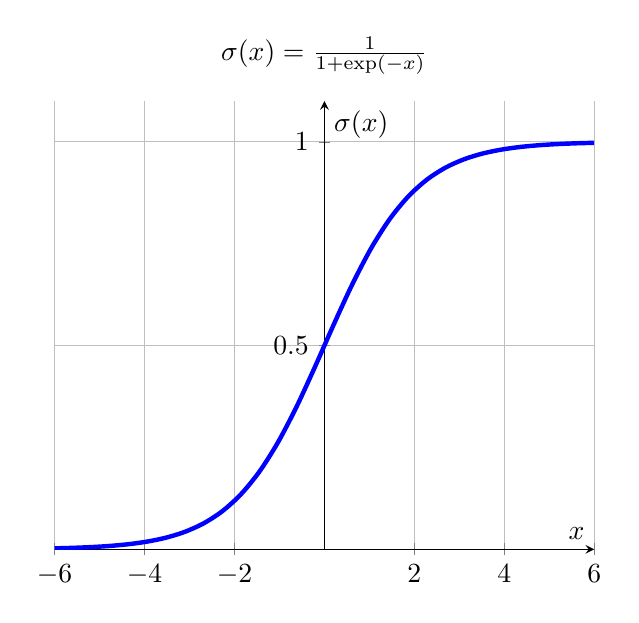
\begin{tikzpicture}[
			% Definisci la funzione sigmoide per poterla riutilizzare facilmente
			declare function={sigmoid(\x)=1/(1+exp(-\x));}
		]
		\begin{axis}[
				% Impostazioni dell'asse
				title={$\sigma(x) = \frac{1}{1 + \exp(-x)}$},
				xlabel={$x$},
				ylabel={$\sigma(x)$},
				axis lines=middle, % Assi centrati all'origine
				xmin=-6, xmax=6, % Range sull'asse x
				ymin=0, ymax=1.1, % Range sull'asse y (un po' sopra 1 per chiarezza)
				xtick={-6,-4,-2,0,2,4,6}, % Tick specifici per x
				ytick={0, 0.5, 1}, % Tick specifici per y
				grid=major, % Aggiunge una griglia per riferimento
				domain=-6:6, % Dominio di campionamento della funzione
				samples=30, % Aumenta i campioni per una curva più liscia
			]
			\addplot[
				blue,
				ultra thick, % Spessore della linea
				smooth % Rende la curva più smussata (anche se con 100 campioni è già liscia)
			] {sigmoid(x)};
		\end{axis}
	\end{tikzpicture}
	\caption{Sigmoid function curve}
\end{figure}
At this point, we know that
\begin{equation}
	\Prob(c_i|\mathbf x)=\sigma(a(\mathbf x))
\end{equation}
so, given the parameters $\bmu_1,\bmu_2,p,\Sigma$, we can make prediction by the following decision rule:
\begin{itemize}
	\item Given $\mathbf x\notin D$
	\item if $\Prob(c_1|\mathbf x)>0.5$ the point $\mathbf x$ is in class $c_1$
	\item else, if $\Prob(c_1|\mathbf x)\le0.5$ the point $\mathbf x$ is in class $c_2$
\end{itemize}

The parameters can be found with the maximum likelihood function, we have to introduce some notation to simplify the understanding process, the dataset is denoted:
\begin{equation}
	D=\{(\mathbf x_n,t_n)_{n=1}^N\}
\end{equation}
where $t_n=1$ if $\mathbf x_n$ is in class $c_1$, else $t_n=0$. This encoding is useful to write the likelihood function. We denote $\mathbf t=(t_n)_{n=1}^N$ the binary vector of the dataset's labels. The likelihood function is the probability that, given the parameters, the labels $\mathbf t$ are correct predictions:
\begin{equation}
	\Prob(\mathbf t|p,\bmu_1,\bmu_2,\Sigma,D)=\prod_{n=1}^{N}
	\left(
	p\mathcal N(\mathbf x_n,\bmu_1,\Sigma)
	\right)^{t_n}
	\left(
	(1-p)\mathcal N(\mathbf x_n,\bmu_2,\Sigma)
	\right)^{(1-t_n)}
\end{equation}

The ML solution is given by the parameters that maximize that function (we use the natural logarithm):
\begin{equation}
	\hat p,\hat\bmu_1,\hat\bmu_2,\hat\Sigma=\arg\max_{p,\bmu_1,\bmu_2,\Sigma}\ln\Prob(\mathbf t|p,\bmu_1,\bmu_2,\Sigma,D)
\end{equation}

In this context the function is analytical and we have a closed form solution, the parameters that maximize that function are
\begin{align}
	 & \hat p=\frac{N_1}{N}, \ \ \ \text{ where } N_1=|\{(\mathbf x,t)\in D \ : \ t=1\}| \\
	 & \hat\bmu_1=\frac{1}{N_1}\sum_{n=1}^Nt_n\mathbf x_n                                \\
	 & \hat\bmu_2=\frac{1}{N_2}\sum_{n=1}^N(1-t_n)\mathbf x_n                            \\
\end{align}

The matrix $\Sigma$ needs the definition of the two matrices\begin{align}
	 & S_1=\frac{1}{N_1}\sum_{(\mathbf x_n,t_n)\in D \ : \ t_n=1}(\mathbf x_n-\hat \bmu_1)(\mathbf x_n-\hat \bmu_1)^T \\
	 & S_2=\frac{1}{N_1}\sum_{(\mathbf x_n,t_n)\in D \ : \ t_n=0}(\mathbf x_n-\hat \bmu_2)(\mathbf x_n-\hat \bmu_2)^T
\end{align}
then
\begin{align}
	 & \hat \Sigma = \frac{N_1}{N}S_1+\frac{N_2}{N}S_2
\end{align}
note that the with $(\mathbf x_n-\hat \bmu_i)(\mathbf x_n-\hat \bmu_i)^T$ is denoted the matrix multiplication between a $d\times 1$ matrix and a $1\times d$ matrix.
\bigskip

The function $a(\mathbf x)$ includes non linear terms, since it includes the Gaussian distribution, apparently, is a non linear function. The following statement is crucial.
\begin{theorem}
	the function $a(\mathbf x)$ is linear in $\mathbf x$:
\end{theorem}
\begin{equation}
	a(\mathbf x)=\mathbf w^T\mathbf x+w_0
\end{equation}
where
\begin{itemize}
    \item $a(\mathbf x)$ measures how much more likely $\mathbf x$ is to come from class $c_1$ than from class $c_2$.
    \item $\mathbf w$ controls the \textbf{orientation} of the decision boundary.
    \item $w_0$ controls the \textbf{position} (or shift) of that boundary.
    \item The condition $a(\mathbf x)=0$ defines a \textbf{linear separating hyperplane} between the two Gaussian classes.
\end{itemize}

\subsection{Models for $k$ Classes}
In this case we have a target function\begin{equation}
	f:X\rightarrow\{c_1,c_2\dots,c_K\}
\end{equation}
we encode the dataset as follows\begin{equation}
	D=\{(\mathbf x_n,\mathbf t_n)\}_{n=1}^N
\end{equation}
where $\mathbf t_n=(t_{n1},\dots t_{nK})$ and $t_{nk}=1\iff$ the $n$-th sample is labeled as class $c_k$.\begin{equation}
	t_{nk}=1\iff f(\mathbf x_n)=c_k
\end{equation}
we estimate $\Prob(c_k|\mathbf x)$ as follows:\begin{equation}
	\Prob(c_k|\mathbf x)=\frac{\Prob(\mathbf x|c_k)\Prob(c_k)}{\sum_{j=1}^K\Prob(\mathbf x|c_j)\Prob(c_j)}=\frac{\exp(a_k)}{\sum_{j=1}^K\exp(a_j)}
\end{equation}
where\begin{equation}
	a_j=\ln\left(\Prob(\mathbf x|c_j)\Prob(c_j)\right)
\end{equation}
we assume that $\Prob(\mathbf x|c_k)$ is Gaussian\begin{equation}
	\Prob(\mathbf x|c_k)=\mathcal N(\mathbf x,\bmu_k,\Sigma)
\end{equation}
and for each class $c_k$, we have that\begin{equation}
	\Prob(c_k)=p_k
\end{equation}
where \begin{equation}
	\sum_{j=1}^Kp_j=1
\end{equation}
so the parameters of the model are\begin{align}
	 & p_1,p_2,\dots p_K\in \R          \\
	 & \bmu_1,\bmu_2\dots \bmu_K\in\R^d \\
	 & \Sigma\in Mat(d\times d)
\end{align}
denoting $\mathbf t$ the set of labels in $D$\begin{equation}
	\mathbf t = \begin{pmatrix}
		\mathbf t_1 & \dots & \mathbf t_N
	\end{pmatrix}
\end{equation}
the maximum likelihood solution is given by:\begin{equation}
	\hat p_1,\dots \hat p_k,\hat \bmu_1,\dots \hat \bmu_k,\hat \Sigma=\arg\max_{p_k,\bmu_k,\Sigma}\ln\left(
	\Prob(\mathbf t|p_1,\dots p_k,\bmu_1,\dots \bmu_k,\Sigma)
	\right)
\end{equation}
the solution can be found analytically and is\begin{align}
	 & \hat p_k=\frac{N_k}{N}\text{ where }N_k=|\{(\mathbf x_n,\mathbf t_n)\in D \ : \ t_{nk}=1\}| \\
	 & \hat\bmu_k=\frac{1}{N_k}\sum_{n=1}^Nt_{nk}\mathbf x_n                                       \\
	 & S_k=\frac{1}{N_k}\sum_{n=1}^Nt_{nk}(\mathbf x_n-\hat\bmu_k)(\mathbf x_n-\hat\bmu_k)^T       \\
	 & \hat \Sigma = \sum_{k=1}^{K}\frac{N_k}{N}S_k
\end{align}
a new sample $\mathbf x'\notin D$ can be predicted as follows:\begin{equation}
	h^*(\mathbf x')=\arg\max_k\frac{\exp(a_k)}{\sum_j\exp(a_j)}
\end{equation}
where $a_k=\ln\left(\hat p_k\mathcal N(\mathbf x',\hat\bmu_k,\hat\Sigma)\right)$.
\subsection{Naive Bayes Assumption}
We can consider an ulterior assumption, that the features of the samples are conditional independent, given a sample $\mathbf x_n\in \R^d$:\begin{equation}
	\Prob(\mathbf x_n|c_k)=\prod_{j=1}^d\Prob(x_{nj}|c_k)
\end{equation}
in this case, for each class $c_k$, we don't have a multivariate Gaussian distribution $\mathcal N(\mathbf x_n,\bmu_k,\Sigma)$, but we have $d$ one-dimensional Gaussian distribution\begin{equation}
	\Prob(x_{nj}|c_k)=\mathcal N(x_{nj},\mu_{jk},\sigma_{jk})
\end{equation}so the parameters of the model are
\begin{equation}
	\begin{matrix}
		p_k\in\R       \\
		\mu_{jk}\in \R \\
		\sigma_{jk}\in \R
	\end{matrix} \ \text{ where } \
	\begin{matrix}
		j=1,\dots d \\ k=1,\dots K
	\end{matrix}
\end{equation}
the maximum likelihood solution can be found analytically:\begin{align}
	 & \hat p_k=\frac{N_k}{N}                                    \\
	 & \hat\mu_{jk}=\frac{1}{N_k}\sum_{n=1}^Nt_{nk}x_{nj}        \\
	 & \hat\sigma_{jk}=\sum_{n=1}^Nt_{nk}(x_{nj}-\hat\mu_{jk})^2
\end{align}
\subsubsection{About the Number of Parameters}
Given a classification problem$$f:\R^d\rightarrow\{c_1\dots c_K\}$$
what are the size (number of parameters) of the generative model? We have the probabilities$$\Prob(c_k)=p_k $$ this counts as $K-1$ parameters, since the first $K-1$ can be used to calculate $p_K$\begin{equation}
	p_K=1-\sum_{k=1}^{K-1}p_k
\end{equation}
then we have $K$ vectors $\bmu_K$, of each $k$-th Gaussian distribution, since each vector have $d$ real components, we have a total of $kd$ parameter. In the end, we have
\section{Discriminative Models}


\chapter{Linear Models}
A linear function on $\mathbf x$ is represented as follows\begin{equation}
	\mathbf w^T\mathbf x+w_0
\end{equation}
we want to use a compact notation, adding a component to the vector $\mathbf x$:\begin{align}
	 & \mathbf x \in \R^d\longrightarrow \tilde{\mathbf x}\in \R^{d+1} \\
	 & \mathbf x=\begin{pmatrix}
		             x_1 & \dots x_d
	             \end{pmatrix}^T                                       \\
	 & \tilde{\mathbf x}=\begin{pmatrix}
		                     1 & x_1 & \dots x_d
	                     \end{pmatrix}^T                           \\
	 & \tilde{\mathbf w}=\begin{pmatrix}
		                     w_0 & w_1 & \dots w_d
	                     \end{pmatrix}^T
\end{align}
so\begin{equation}
	\mathbf w^T\mathbf x +w_0=\tilde{\mathbf w}^T\tilde{\mathbf x}=w_0+w_1x_1\dots w_dx_d.
\end{equation}
In general, we have an error function $E(\mathbf w)$ that we want to minimize\begin{equation}
	\mathbf w^*=\arg\min_{\mathbf w}E(\mathbf w)
\end{equation}

% Bibliography and citation part, actually unused, keeped for compilation errors
%
\bibliographystyle{plain}   % or abbrv/unsrt etc.
\bibliography{references}   % references.bib must exist
\cite{} % needed to fix "found no citation error"
%
%

\end{document}